%!TEX program = xelatex
% 完整编译: xelatex -> bibtex -> xelatex -> xelatex
\documentclass[lang=cn,11pt,a4paper,cite=super]{elegantpaper}

\title{这蘑菇有毒!}
\author{蒋文馨 \quad 16342067 \quad
   \email{jiangwx7@mail2.sysu.edu.cn}}
\institute{中山大学数学学院17级统计学}
\date{\zhtoday}


% 本文档命令
\usepackage{array}
\usepackage{caption}
\usepackage{subcaption}
\newcommand{\ccr}[1]{\makecell{{\color{#1}\rule{1cm}{1cm}}}}

\begin{document}
\maketitle
\thispagestyle{empty}
\begin{abstract}
   本文基于UCI蘑菇数据集,建立判别蘑菇是否可食用的分类器。
   数据集样本量为8124,其中可食用和不可食用分别为4208和3916,
   自变量有22个,均为因子型变量。
   首先对数据进行详细的探索性分析。对于缺失值,尝试决策树、多重填补
   和kNN三种填补方法,最终选用kNN对训练集和测试集分别进行填补。
   之后,根据模型需求,将因子型变量编码为哑变量。
   使用主成分回归 、线性判别分析、 LASSO 回归 、逐步回归、
   决策树(CART、 C4.5、 C5.0)、 随机森林、 XGBoost、
   kNN、 SVM 、NN、 RIPPER 和PART,共14种模型
   建立了性能优秀的分类器,并基于树模型给出了特征的重要性。
   \keywords{Mushroom \quad 缺失值 \quad LASSO回归 \quad 随机森林 \quad 
   XGBoost \quad  NN}
\end{abstract}
%\newpage
%\setcounter{page}{1}
\setcounter{tocdepth}{1}
\tableofcontents
\thispagestyle{empty}
\newpage

\setcounter{page}{1}
\setcounter{section}{-1}

\section{注释}
本文基于我多元统计期末大作业,有删改。

\section{引言}\label{sec:0}
每年都有很多人因为摄入有毒野生蘑菇生病,甚至死亡~\cite{zhongdu}。由于许多蘑菇在外观上非常相似,
所以即使是有经验的蘑菇采集者也会中毒。百度百科上鉴别有毒蘑菇的方法为~\cite{baike}:
\begin{enumerate}
   \itemsep = 0pt
   \item 观形状,毒蘑 菇般比较黏滑,菌盖上常黏些杂物,或生长一些像补丁状的斑块,菌柄上常有菌环;
      无毒蘑菇很少有菌环。
   \item 察色味,有毒磨菇的颜色比较浓艳,菌伞带有红、紫、黄或其他杂色斑点,基底红色,形状异常;
      无毒蘑菇为苦杏或水果味。毒蘑菇有土豆或萝卜味,而且有辛辣、恶臭和苦味。
   % \item 看分泌物,将采摘的新鲜野蘑菇撕断菌杆,无毒的分泌物清亮如水,个别为白色,菌面撕断不变色;
   %    有毒的分泌物稠浓,呈赤褐色,撕断后在空气中易变色。
   \item \dots
\end{enumerate}

本文使用UCI机器学习库的Mushroom数据集,完成以下两个任务:
\begin{itemize}
   \item 建立判断野生蘑菇是否可食用的分类器;
   \item 探究蘑菇是否可食用与哪些特征相关。
\end{itemize}
需要注意的是,关于毒蘑菇的识别,迄今为止还没有找到一种既科学可靠,又简单易行的具体适用方法~\cite{jianbie}。
所以,为确保安全,\textbf{不建议食用野生蘑菇}。

\section{数据说明}
本文所用数据集属于UCI机器学习库的Mushroom数据集\footnote{也是XGBoost安装包中的demo数据集}。
本文使用Kaggle版数据\footnote{Kaggle版的优势在于拥有表头},网址为 \url{https://www.kaggle.com/uciml/mushroom-classification}。
该数据集包括了列于《 Audubon Society Field Guide to North American Mushrooms (1981)》
上的23个带菌褶的磨菇品种的8124个磨菇案例信息。在食用指南中,每种蘑菇被鉴定为
肯定可以食用”,“肯定是有毒的”和“可能有毒,不建议食用”。
“可能有毒,不建议食用”和“肯定是有毒的”合并到一起,形成最终的两个类:
不可食用(poisonous)和可食用(edible),分别有4208和3916个样本。

因数据集只记录了北美 Agaricus 和 Lepiota 科的蘑菇信息,许多常见蘑菇种类及特征未包含在数据集中,
所以不建议将本文所得模型用于判断其它地区或其它科蘑菇是否可食用。

\section{探索性分析}
首先,对数据集进行概述。然后,再分别介绍每一个特征。
\begin{enumerate}
   \itemsep = 10pt
   \setcounter{enumi}{-1}
   \item 数据概览:\par 总样本数为8124。特征包括1个因变量和22个自变量,
   均为名义型变量,在R中储存为因子型变量。缺失值只存在于自变量菌托(stalk.root)中,用“?”表示 。
   缺失情况说明见\ref{item:1},对缺失值的处理见 \ref{sec:missingdata}。
   变量的中英文对照及取值见表\ref{tab:sjgl},示意图如图\ref{fig:syt}所示。
   表格中的取值为可能取值的简写,实际取值是可能取值的子集,例如菌褶剖面4种可能取值为a,d,f,n,
   但数据集中菌褶剖面只有a,f这2种取值。菌幕性状包括菌托和菌环的情况。
   \begin{table}[hbt]
      \centering
      \caption{数据概览}
      \label{tab:sjgl}
      \setlength{\tabcolsep}{7mm}{
      \begin{tabular}{llll} 
      \toprule
      序号 & 英文名                      & 中文名    & 取值                      \\
      \midrule
      1  & class                    & 类别     & e,p                      \\
      2  & cap.shape                & 菌盖形状   & b,c,x,f,k,s              \\
      3  & cap.surface              & 菌盖表面特征 & f,g,y,s                  \\
      4  & cap.color                & 菌盖颜色   & n,b,c,g,r,p,u,e,w,y      \\
      5  & bruises                  & 擦伤反应   & t,f                      \\
      6  & odor                     & 气味     & a,l,c,y,f,m,n,p,s        \\
      7  & gill.attachment          & 菌褶剖面   & a,d,f,n                  \\
      8  & gill.spacing             & 菌褶间隔   & c,w,d                    \\
      9  & gill.size                & 菌褶大小   & b,n                      \\
      10 & gill.color               & 菌褶颜色   & k,n,b,h,g,r,o,p,u,e,w,y  \\
      11 & stalk.shape              & 菌柄形状   & e,t                      \\
      12 & stalk.root               & 菌托     & b,c,u,e,z,r,?            \\
      13 & stalk.surface.above.ring & 环上柄面   & f,y,k,s                  \\
      14 & stalk.surface.below.ring & 环下柄面   & f,y,k,s                  \\
      15 & stalk.color.above.ring   & 环上柄色   & n,b,c,g,o,p,e,w,y        \\
      16 & stalk.color.below.ring   & 环下柄色   & n,b,c,g,o,p,e,w,y        \\
      17 & veil.type                & 菌幕类型   & p,u                      \\
      18 & veil.color               & 菌幕颜色   & n,o,w,y                  \\
      19 & ring.number              & 菌环数量   & n,o,t                    \\
      20 & ring.type                & 菌环类型   & c,e,f,l,n,p,s,z          \\
      21 & spore.print.color        & 孢子印颜色  & k,n,b,h,r,o,u,w,y        \\
      22 & population               & 生长分布   & a,c,n,s,v,y              \\
      23 & habitat                  & 生长环境    & g,l,m,p,u,w,d            \\
      \bottomrule
      \end{tabular}}
   \end{table}
   \begin{figure}[!hbt]
      \centering
      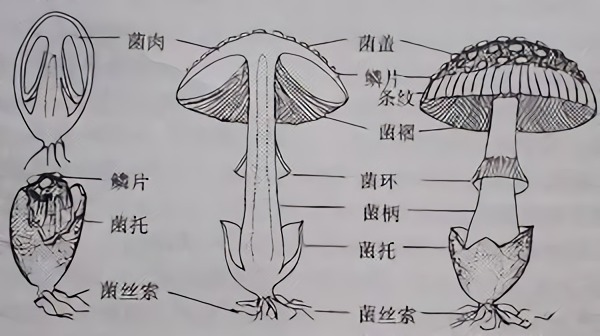
\includegraphics[width=0.6\linewidth]{img/syt.jpg}
      \caption{蘑菇结构示意图}
      \label{fig:syt}
   \end{figure}
   
   \item 类别:\par
   类别变量为分析的目标变量,有2种取值,分别为:可食用(edible=e),样本数为4208个,占比为51.8\%;
   不可食用(poisonous=p),样本数为3916个,占比为48.2\%,如图\ref{fig:class}所示。
   可以看出两种类型数目大致相当,数据平衡。
   \begin{figure}[!hbt]
      \centering
      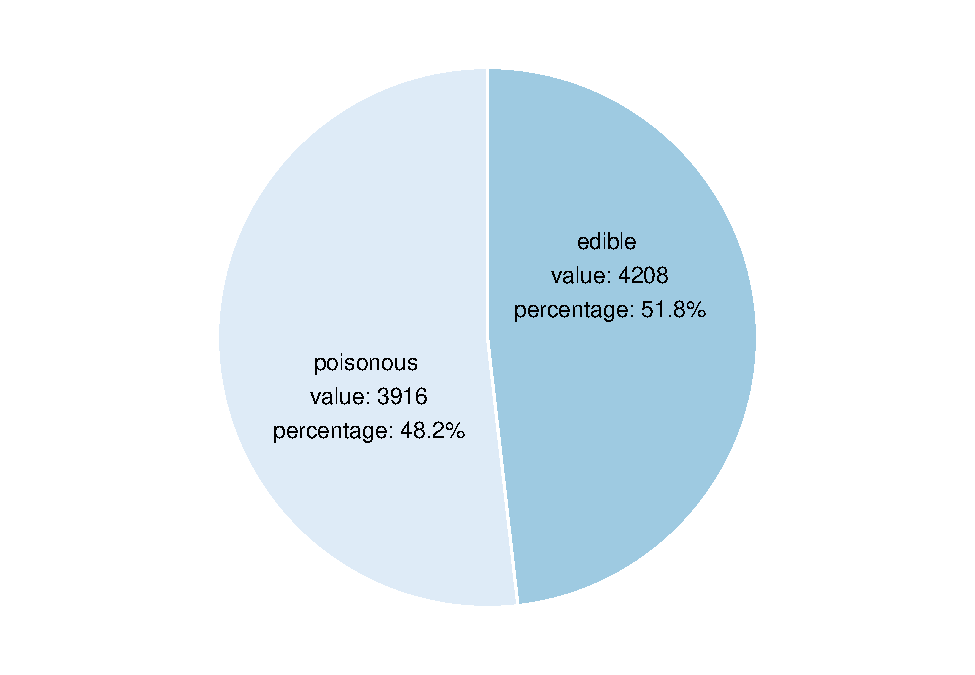
\includegraphics[width=0.6\linewidth]{img/class_pie-1.pdf}
      \caption{类别的分布情况}
      \label{fig:class}
   \end{figure}
   
   \item 菌盖形状:\par 有6种取值,分别为bell=b,conical=c,convex=x,flat=f,
   knobbed=k,sunken=s(等号表示缩写后符号,下同),如图\ref{fig:capshape}所示
   \footnote{图片由ggplot2在Rmd中绘制并生成pdf文件,示意图来自网络~\cite{pic}}。
   \begin{figure}[hbt]
      \begin{subfigure}[b]{0.69\textwidth}
        \centering
        % include 1 image
        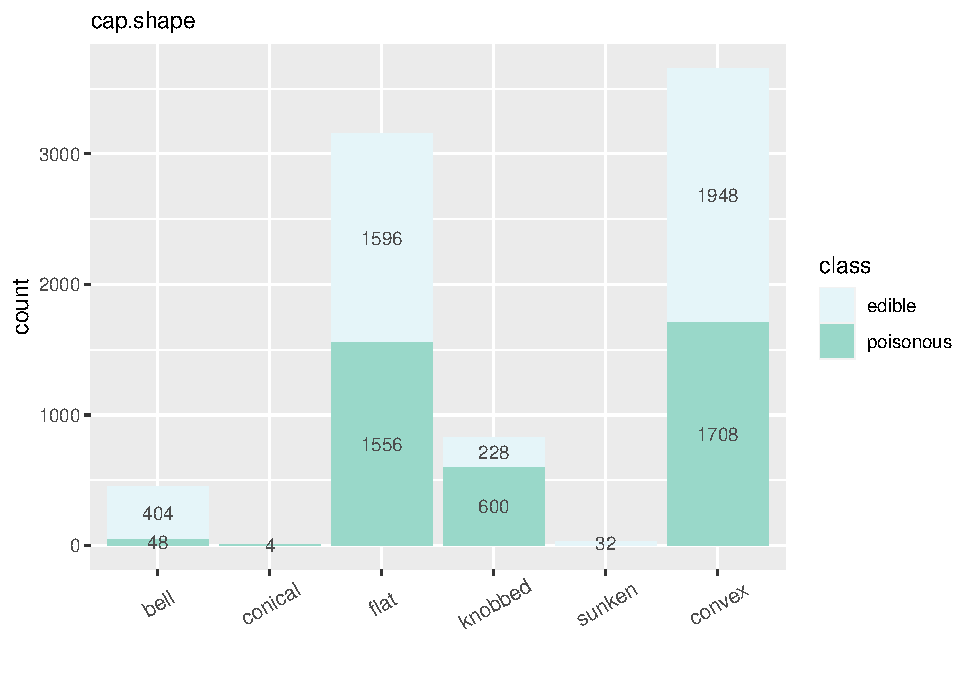
\includegraphics[width=\linewidth]{img/capshape-1.pdf}  
      \caption{菌盖形状分布情况}
      \end{subfigure}
      \begin{subfigure}[b]{0.3\textwidth}
        \centering
        % include 2 image
        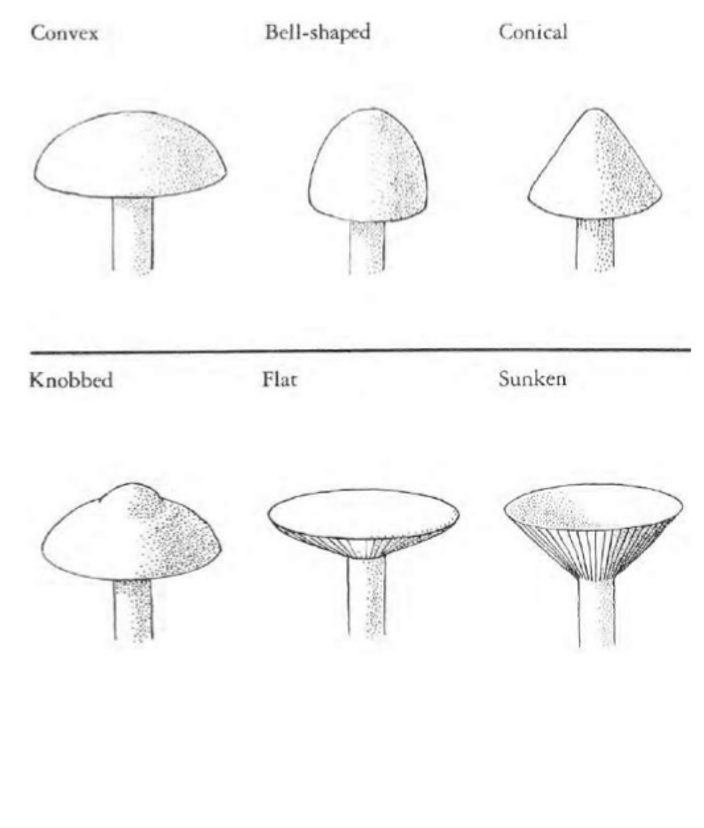
\includegraphics[width=\linewidth]{img/capshape1.PNG}  
        \caption{菌盖形状示意图}
      \end{subfigure}
      \caption{菌盖形状}
      \label{fig:capshape}
   \end{figure}

   \item 菌盖表面特征:\par 有4种取值,分别为 fibrous=f,grooves\footnote{表示菌盖表面有凹槽,未找到相应的图示}
   =g,scaly=y,smooth=s,如图\ref{fig:capsurface}所示。
   \begin{figure}[htb]
      \begin{subfigure}[b]{0.69\textwidth}
        \centering
        % include 1 image
        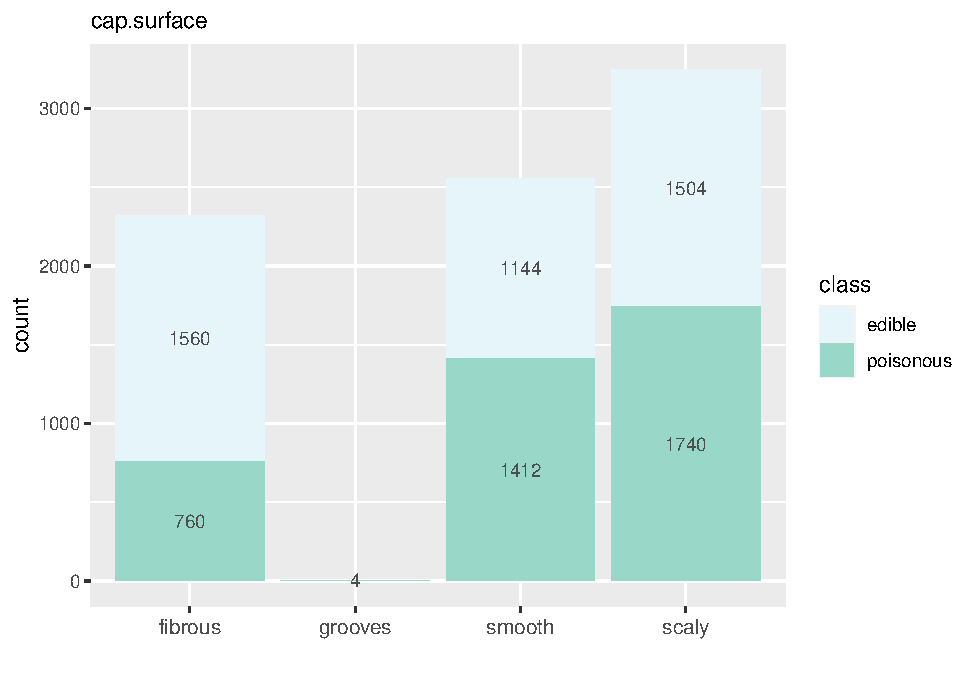
\includegraphics[width=\linewidth]{img/capsurface-1.pdf}  
      \caption{菌盖表面特征分布情况}
      \end{subfigure}
      \begin{subfigure}[b]{0.3\textwidth}
        \centering
        % include 2 image
        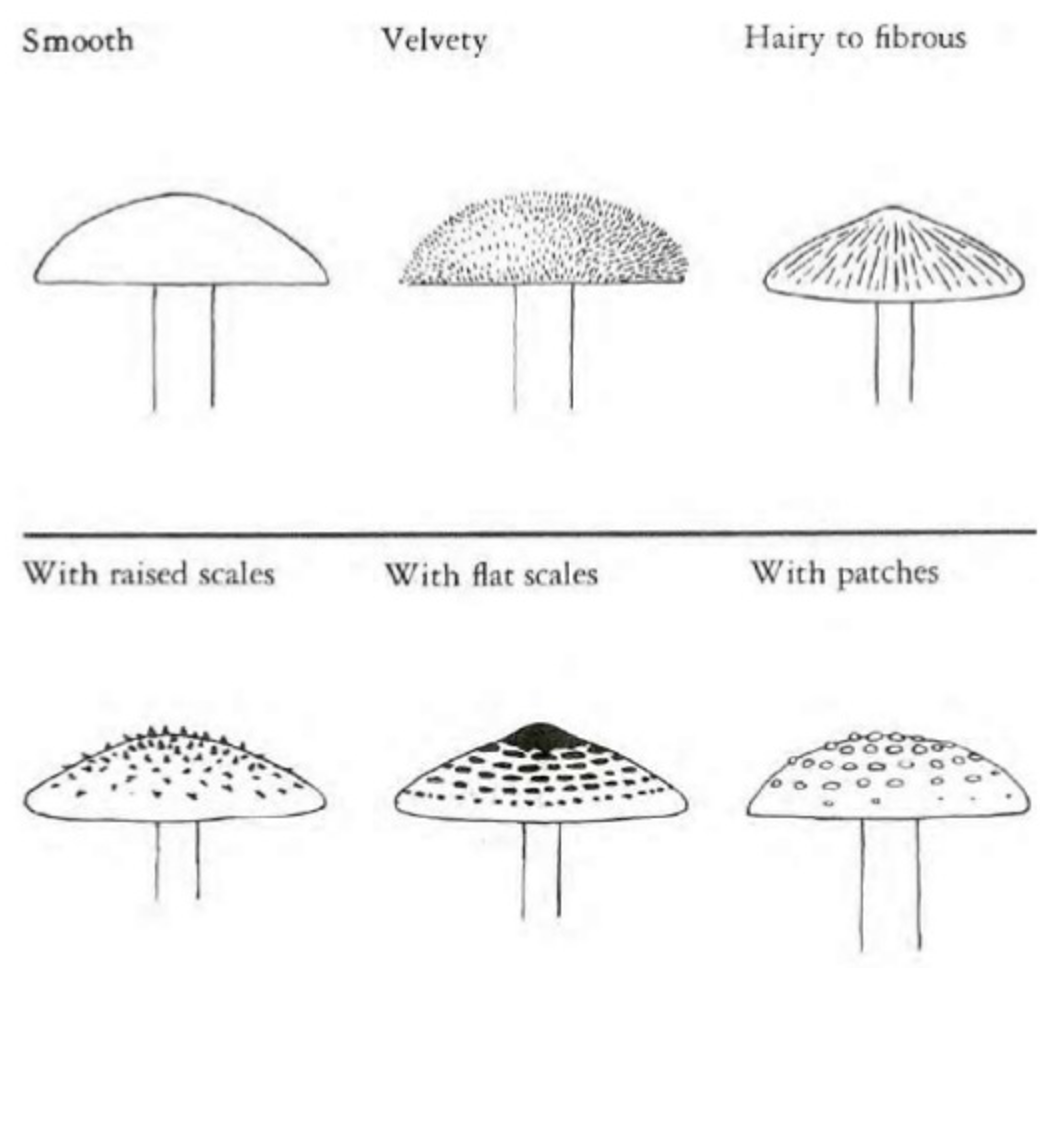
\includegraphics[width=\linewidth]{img/capsurface.PNG}  
        \caption{菌盖表面特征示意图}
      \end{subfigure}
      \caption{菌盖表面特征}
      \label{fig:capsurface}
   \end{figure}
   \item 菌盖颜色:\par 有6种取值,分别为brown=n,buff=b,cinnamon=c,gray=g,
   pink=p,red=e,如图\ref{fig:capsurfacecol}所示。实际颜色与名称的对比如图\ref{fig:truec}所示。
   \begin{figure}[htb]
      \begin{subfigure}[b]{0.69\textwidth}
        \centering
        % include 1 image
        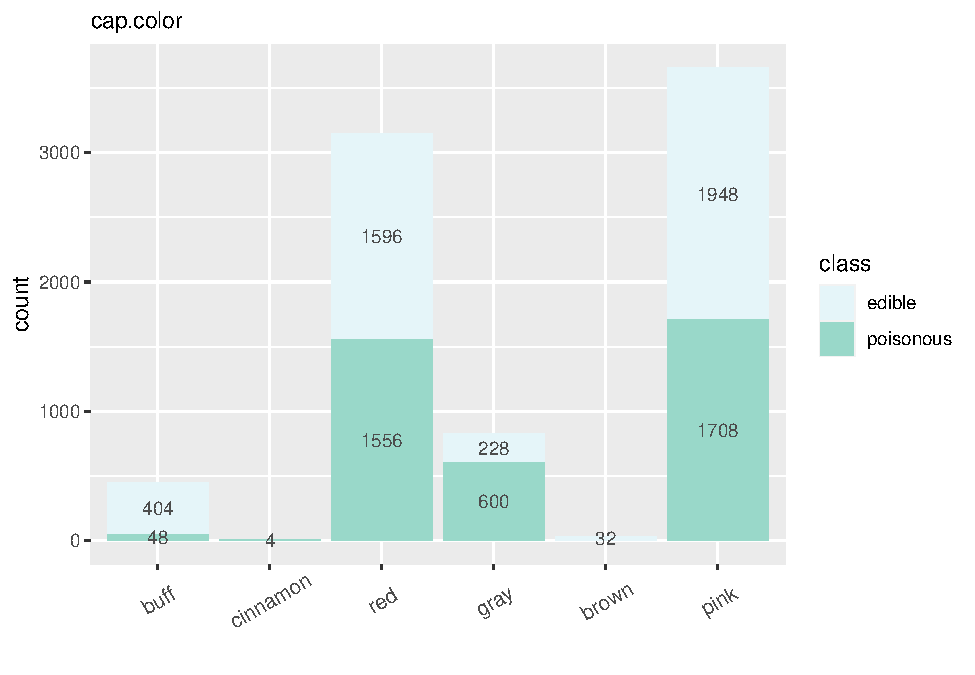
\includegraphics[width=\linewidth]{img/capcolor-1.pdf}  
      \caption{菌盖颜色分布情况}
      \end{subfigure}
      \begin{subfigure}[b]{0.3\textwidth}
        \centering
        % include 2 image
        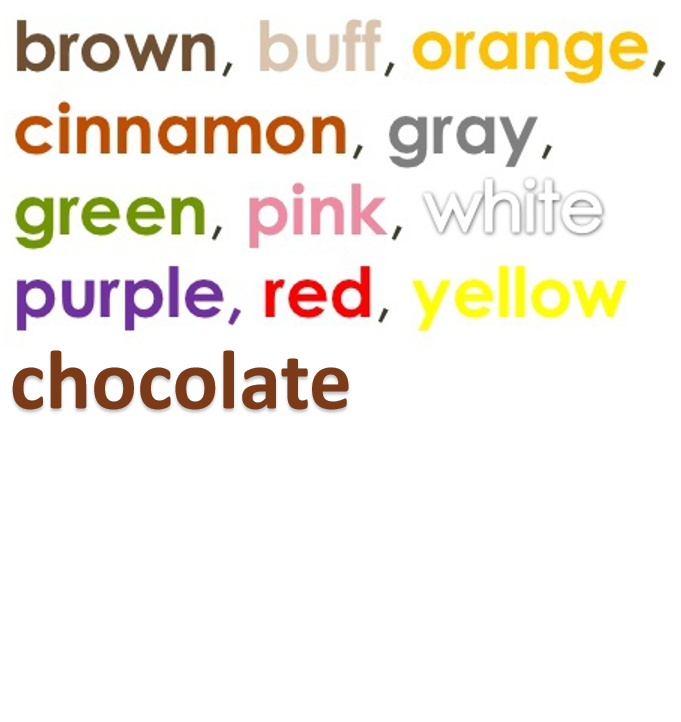
\includegraphics[width=\linewidth]{img/color.PNG}  
        \caption{颜色示意图}
        \label{fig:color0}
      \end{subfigure}
      \caption{菌盖颜色}
      \label{fig:capsurfacecol}
   \end{figure}

   \item 擦伤反应:\par 有2种取值,分别为TRUE表示存在擦伤反应,FALSE表示不存在擦伤反应,如图\ref{fig:bru}所示。
   擦伤反应即当蘑菇受到损伤时,伤口出现的特殊颜色,一般为蓝色或者绿色。
   存在擦伤反应表明该蘑菇含有一些特殊化合物,可能与致幻(即不可食用)相关~\cite{bru}。
   但数据集中大多数可食用蘑菇也存在擦伤反应。
   % \begin{figure}[htb]
   %    \centering
   %    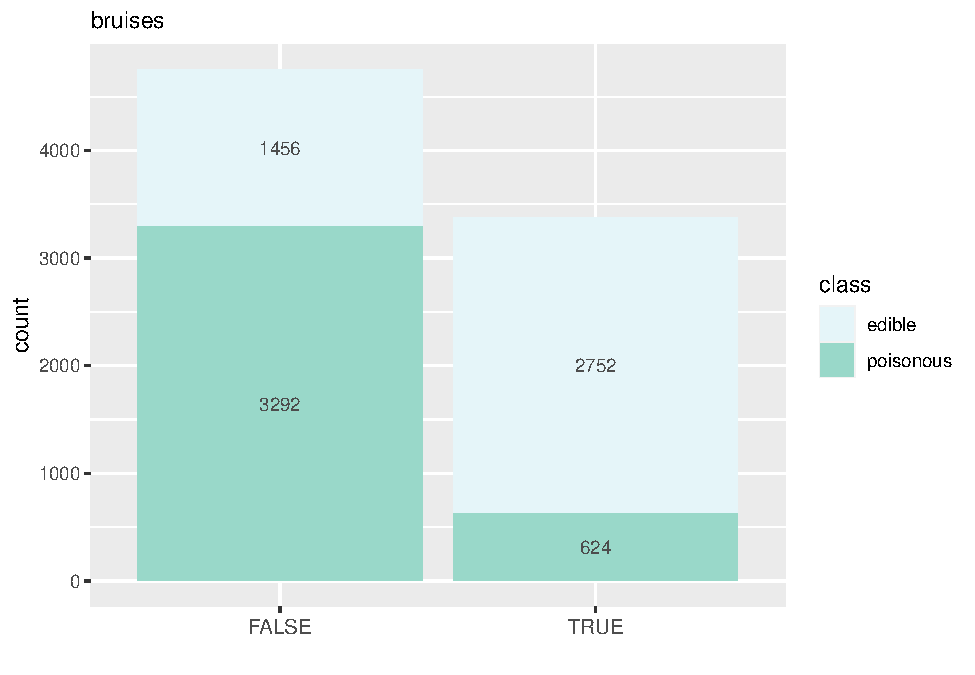
\includegraphics[width=0.7\linewidth]{img/bruises-1.pdf}
   %    \caption{擦伤反应分布情况}
   %    \label{fig:bru}
   % \end{figure}   
   \item 气味:\par 有9种取值,分别为almond=a,anise=l,creosote=c,fishy=y,foul=f,
   musty=m,none=n,pungent=p,spicy=s,如图\ref{fig:odor}所示。可以看出,特殊气味
   与不可食用有很大的相关性。无味(none)基本为可食用菌,但也有例外。因此单凭无味不可以
   断定蘑菇可食用。
   \begin{figure}[htb]
      \begin{subfigure}[t]{0.49\textwidth}
        \centering
        % include 1 image
        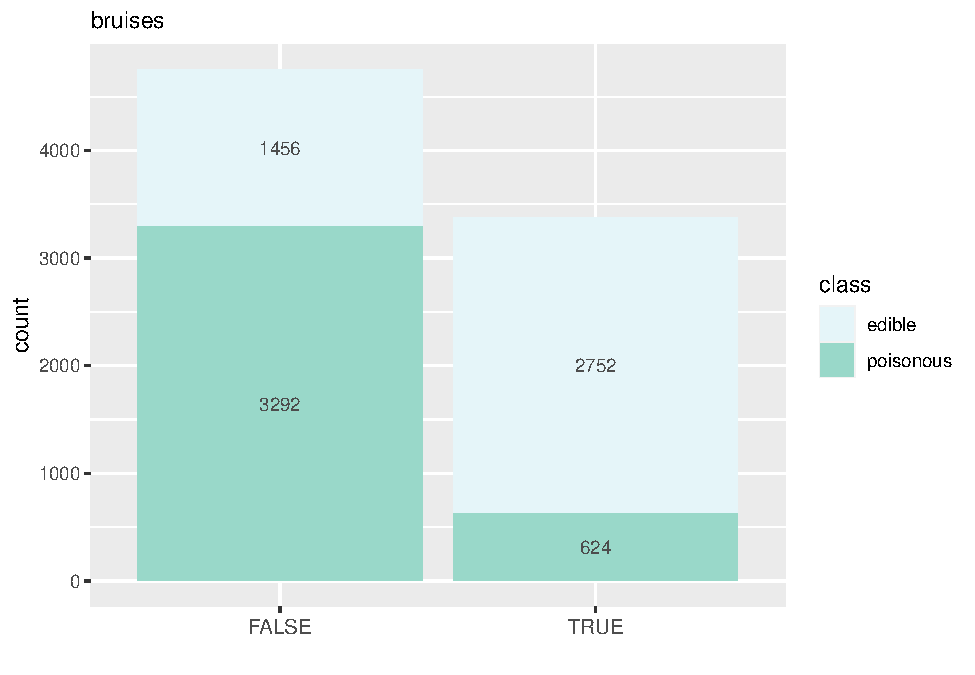
\includegraphics[width=\linewidth]{img/bruises-1.pdf}
      \caption{擦伤反应分布情况}
      \label{fig:bru}
      \end{subfigure}
      \begin{subfigure}[t]{0.50\textwidth}
        \centering
        % include 2 imaget
        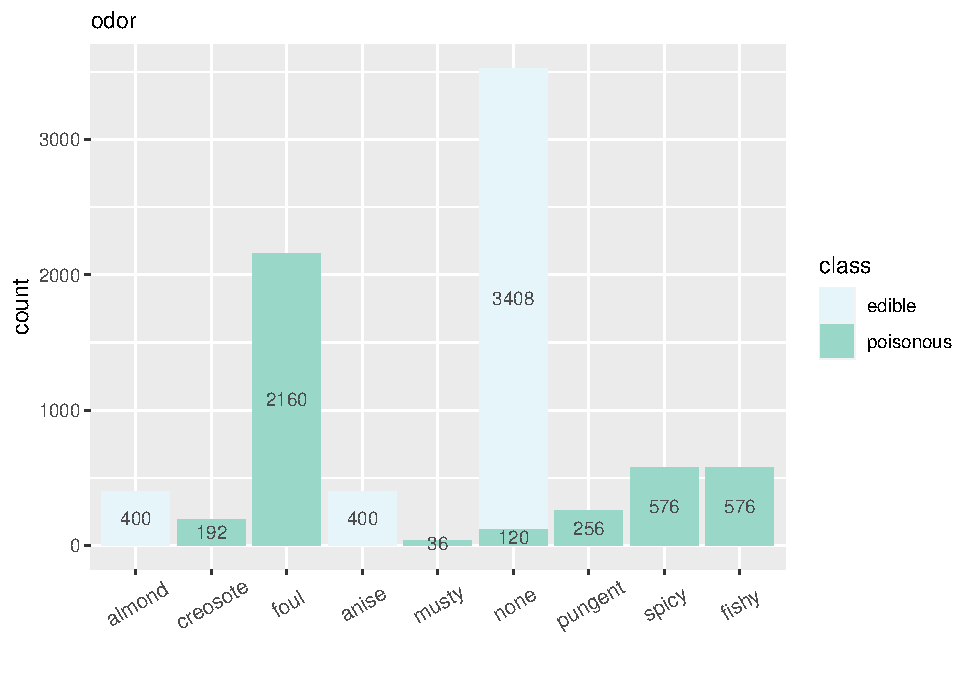
\includegraphics[width=\linewidth]{img/odor-1.pdf} 
        \caption{气味分布情况}
        \label{fig:odor} 
      \end{subfigure}
      \caption{擦伤反应和气味}
   \end{figure}

   % \begin{figure}[htb]
   %    \centering
   %    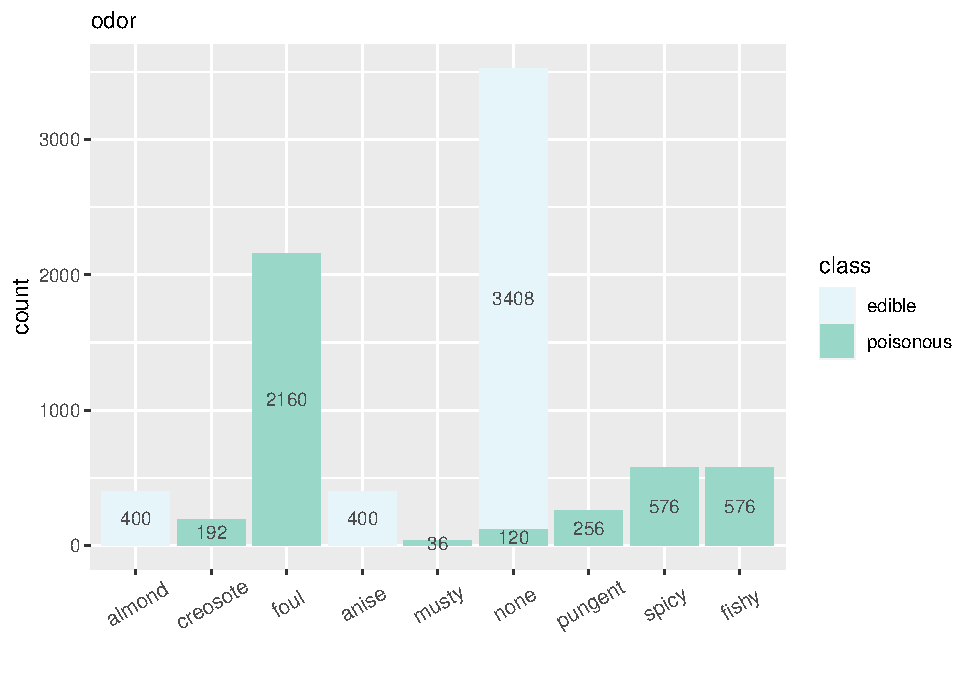
\includegraphics[width=0.7\linewidth]{img/odor-1.pdf}
   %    \caption{气味分布情况}
   %    \label{fig:odor}  
   % \end{figure}
   \item 菌褶剖面:\par 有2种取值,分别为attached=a,free=f,
   如图\ref{fig:gillatt}所示~\cite{mogutujian}。
   \begin{figure}[htb]
      \begin{subfigure}[b]{0.69\textwidth}
        \centering
        % include 1 image
        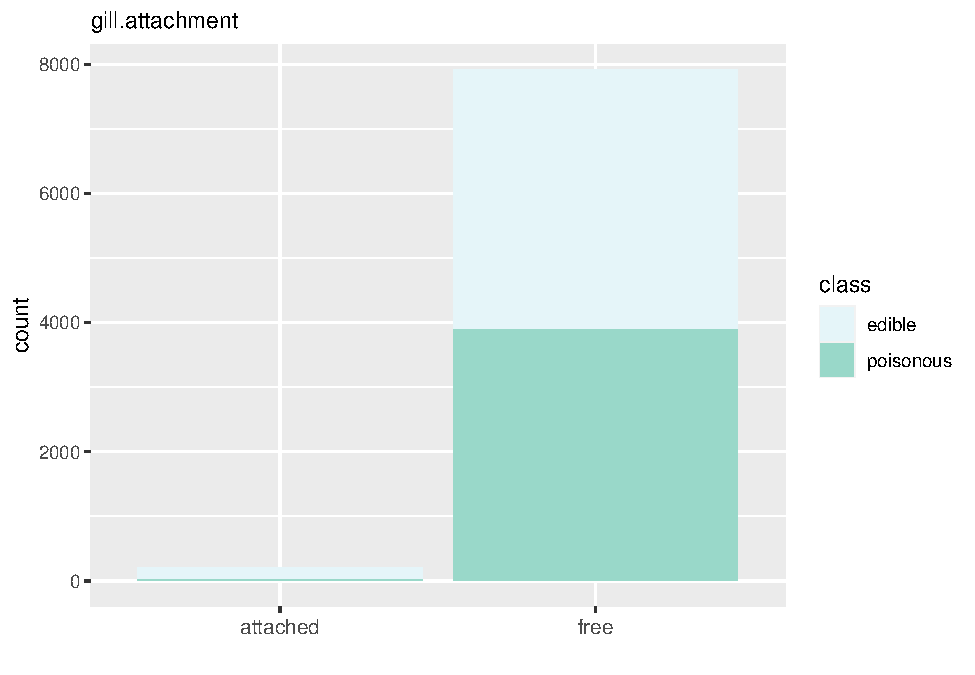
\includegraphics[width=\linewidth]{img/gillattachment-1.pdf}  
      \caption{菌褶剖面分布情况}
      \end{subfigure}
      \begin{subfigure}[b]{0.25\textwidth}
        \centering
        % include 2 image
        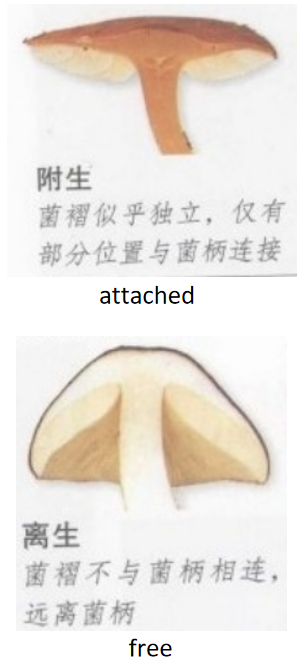
\includegraphics[width=\linewidth,height=3in]{img/gillatt.PNG}  
        \caption{菌褶剖面示意图}
      \end{subfigure}
      \caption{菌褶剖面}
      \label{fig:gillatt}
   \end{figure}

   \item 菌褶间隔:\par 有2种取值,分别为close=c,crowded=w,如图\ref{fig:gillspa}所示。
   可以看出菌褶细、间隔密集的蘑菇大多数是可以食用的。
   \begin{figure}[!bht]
      \begin{subfigure}[b]{0.69\textwidth}
        \centering
        % include 1 image
        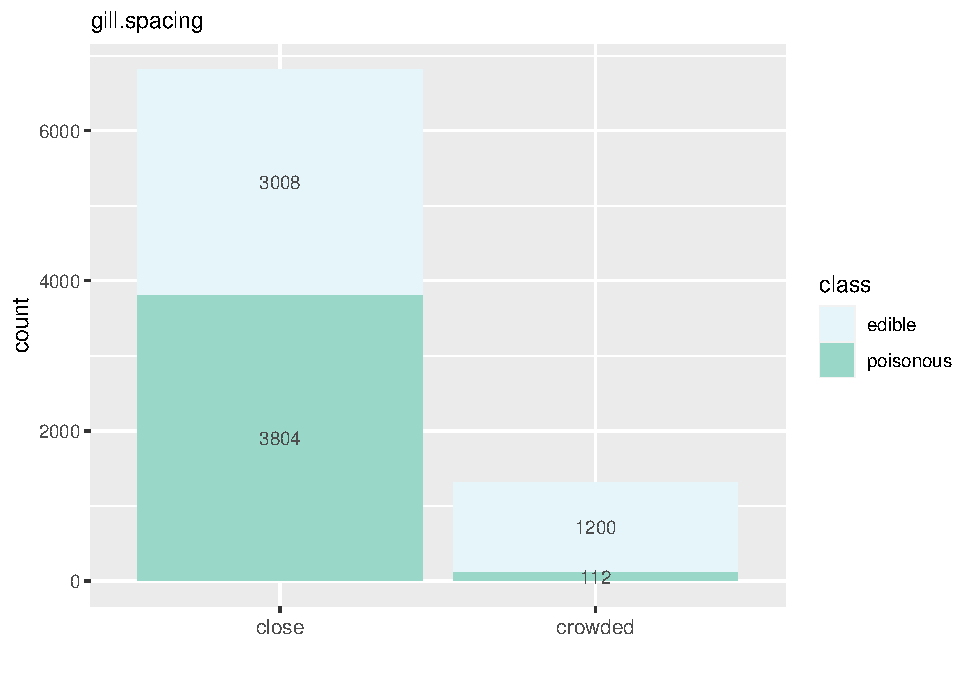
\includegraphics[width=\linewidth]{img/gillspacing-1.pdf}  
      \caption{菌褶间隔分布情况}
      \end{subfigure}
      \begin{subfigure}[b]{0.3\textwidth}
        \centering
        % include 2 image
        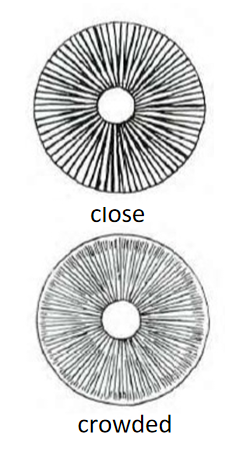
\includegraphics[width=0.9\linewidth,height=3in]{img/gillspac.PNG}  
        \caption{菌褶间隔面示意图}
      \end{subfigure}
      \caption{菌褶间隔}
      \label{fig:gillspa}
   \end{figure}

   \item 菌褶大小:\par 有2种取值,分别为宽间隔(broad=b),稠密(narrow=n),
   如图\ref{fig:gillsi}所示。菌褶稠密的蘑菇大都是不可食用的。
   \begin{figure}[htb]
      \begin{subfigure}[b]{0.69\textwidth}
        \centering
        % include 1 image
        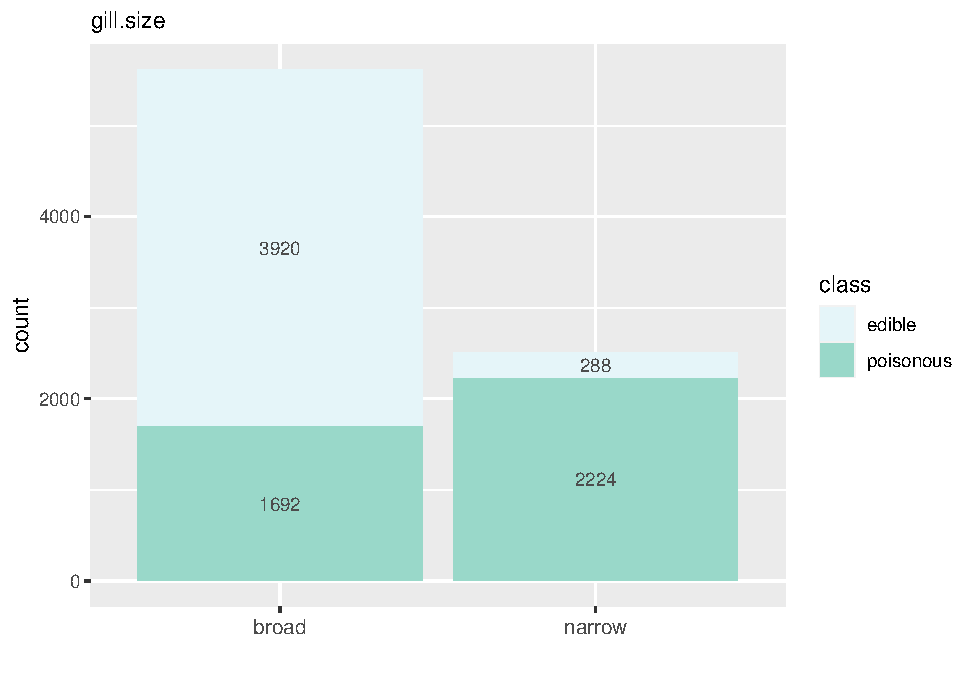
\includegraphics[width=\linewidth]{img/gillsize-1.pdf}  
      \caption{菌褶大小分布情况}
      \end{subfigure}
      \begin{subfigure}[b]{0.3\textwidth}
        \centering
        % include 2 image
        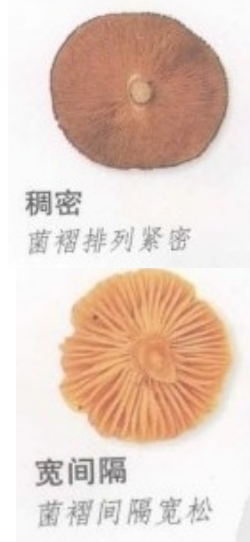
\includegraphics[width=0.8\linewidth,height=2.8in]{img/gillsize.PNG}  
        \caption{菌褶大小面示意图}
      \end{subfigure}
      \caption{菌褶大小}
      \label{fig:gillsi}
   \end{figure}  
   \item 菌褶颜色:\par 有12种取值,分别为black=k,brown=n,buff=b,chocolate=h,gray=g,
   green=r,orange=o,pink=p,purple=u,red=e,
   white=w,yellow=y,如图\ref{fig:gillcol}所示,实际颜色如图\ref{fig:truec}所示。
   菌褶颜色为buff的全部不可食用;而菌褶颜色为red的全部可食用。
   % \begin{figure}[!bht]
   %    \begin{subfigure}[b]{0.69\textwidth}
   %      \centering
   %      % include 1 image
   %      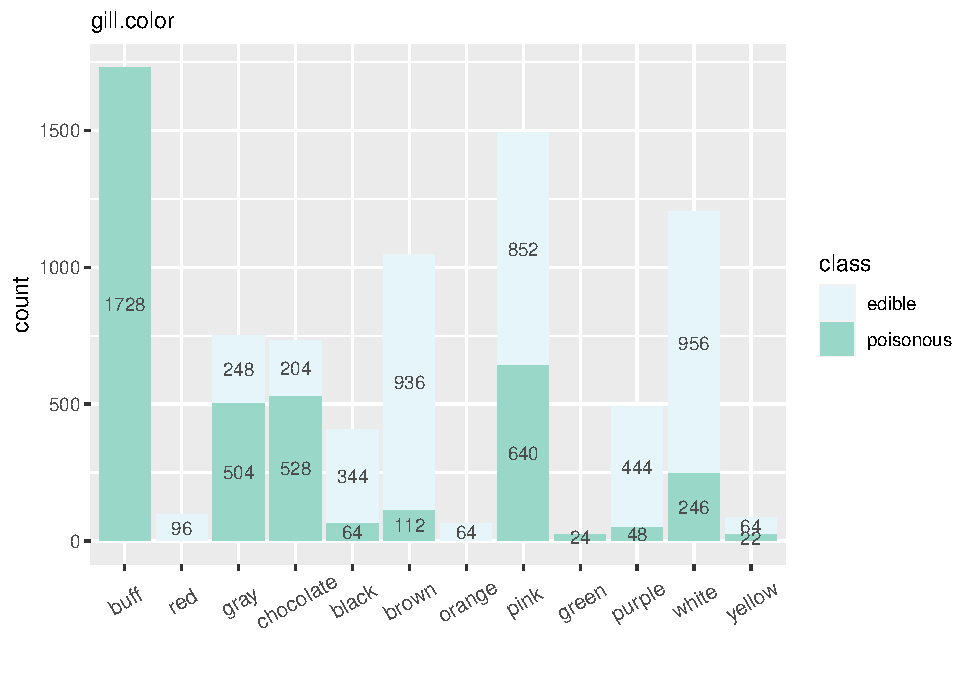
\includegraphics[width=\linewidth]{img/gillcolor-1.pdf}  
   %    \caption{菌褶颜色分布情况}
   %    \end{subfigure}
   %    \begin{subfigure}[b]{0.3\textwidth}
   %      \centering
   %      % include 2 image
   %      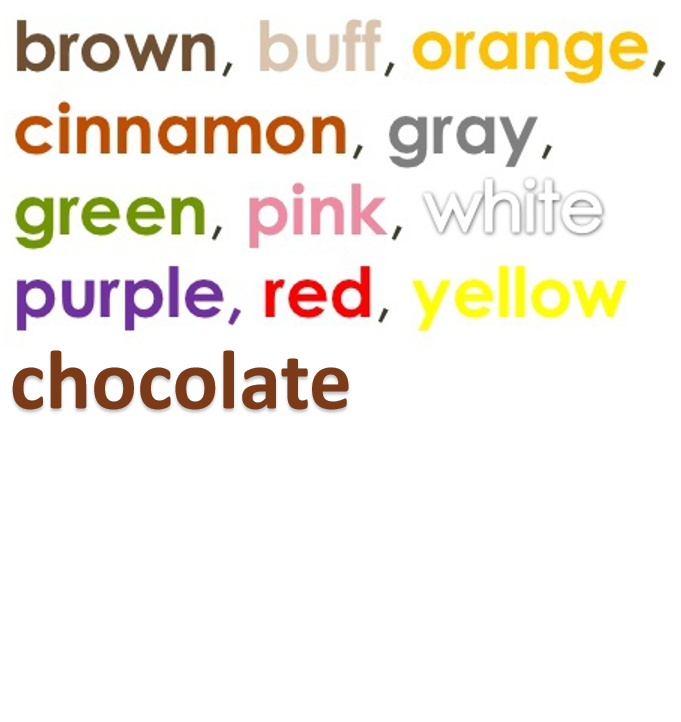
\includegraphics[width=\linewidth]{img/color.PNG}  
   %      \caption{颜色示意图}
   %    \end{subfigure}
   %    \caption{菌褶颜色}
   %    \label{fig:gillcol}
   % \end{figure}
   \begin{figure}[htb]
      \centering
      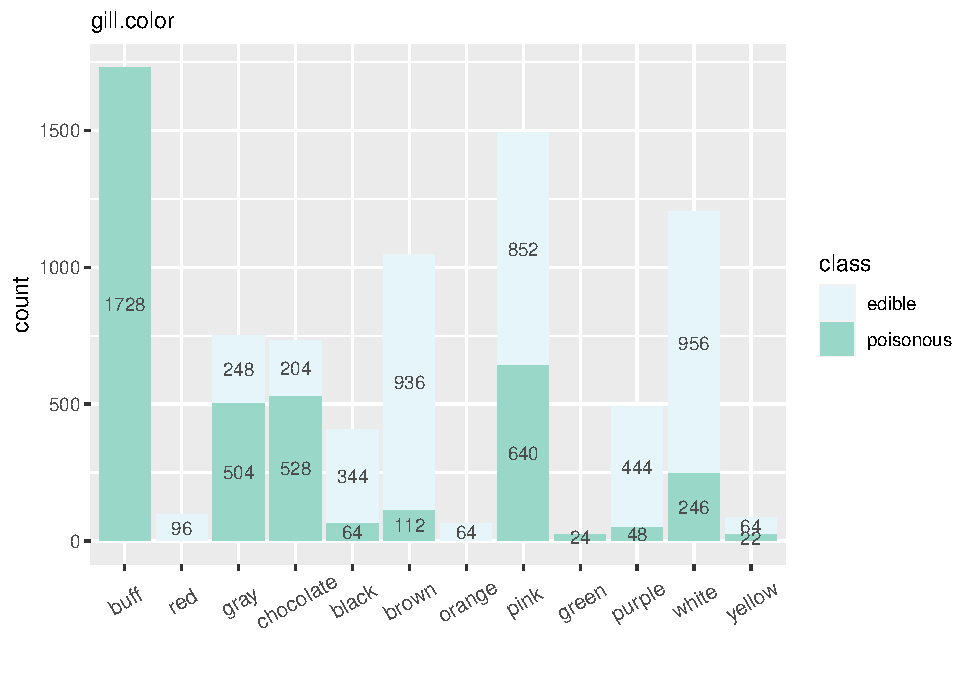
\includegraphics[width=0.8\linewidth]{img/gillcolor-1.pdf} 
      \caption{菌褶颜色分布情况}
      \label{fig:gillcol}
   \end{figure}
   \begin{figure}[!hbt]
      \centering
      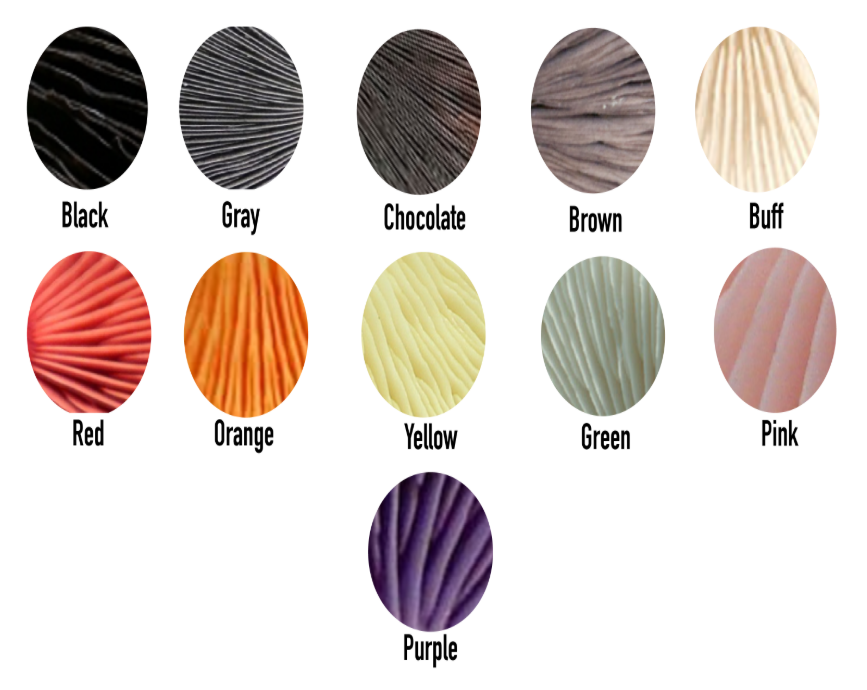
\includegraphics[width=0.65\linewidth]{img/colortrue.PNG}
      \caption{实际颜色对照图}
      \label{fig:truec}
   \end{figure}

   \item 菌柄形状:\par 有2种取值分别为上细下粗(enlarging=e),
   上粗下细(tapering=t),如图\ref{fig:ss}所示。
   \begin{figure}[phtb]
      \centering
      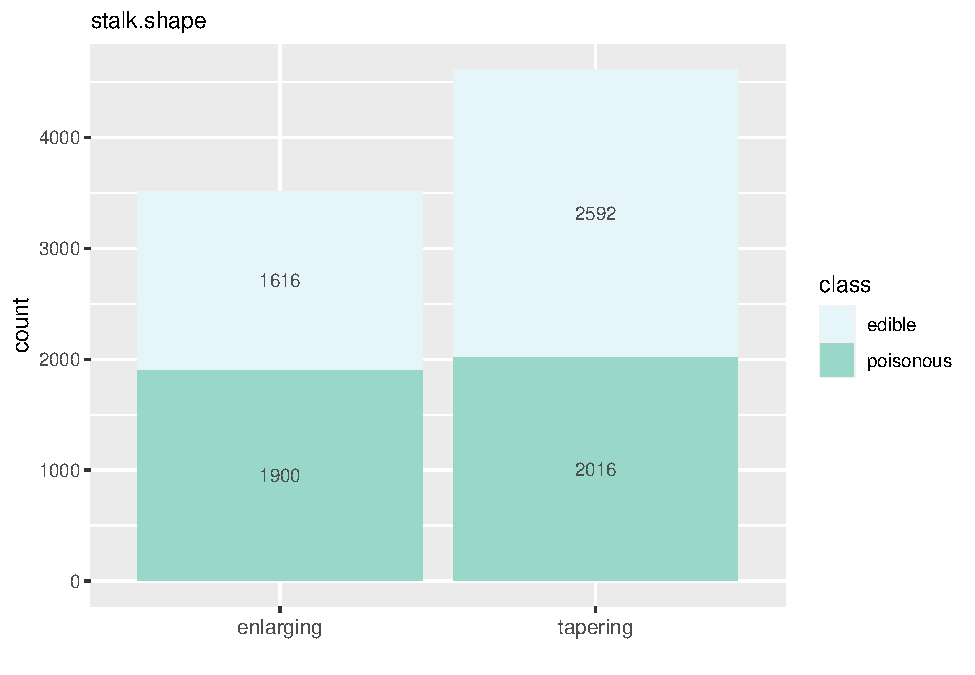
\includegraphics[width=0.7\linewidth]{img/stalkshape-1.pdf}
      \caption{菌柄形状分布情况}
      \label{fig:ss}
   \end{figure}

   \item\label{item:1} 菌托:\par 有5种取值,分别为bulbous=b,club=c,equal=e,
   rooted=r,missing=?,其中“?”表示缺失值,两种类型蘑菇共2480个缺失值,在所有样品中占比超过30\%。
   如图\ref{fig:stalkroot}所示。可以看出,rooted型菌托的蘑菇均可以食用。
   出现缺失值的原因可能为:
   \begin{itemize}
      \item 无法判断菌托类型:从\ref{fig:jtsyt}中可以看出bulbous型和cup型菌托长相相似,很难分辨。
      \item 损伤根部:采集的过程中损伤根部以至于无法判断菌托类型。
      缺失值中不可食用比例高于其它菌托类型,这可能是因为有毒的蘑菇更容易受到损伤。
      \item 蘑菇本身未发育完全。
   \end{itemize}  
   判断缺失类型为完全非随机缺失(Missing Not At Random,MNAR)和任意缺失。
   关于缺失值的介绍及处理在章节\ref{sec:missingdata}   
   \footnote{Kaggle和其他平台上很多解答把“?”当成一个独立的类别,
   因为不处理缺失值,一些分类器(例如基于树的随机森林)依然可以有很好的表现。更何况缺失值中不可食用
   的比例高于其它菌托类型,这有助于分类。但本文认为不处理缺失值是不合理的,即使缺失和不可食用确有关联。}。
   
   \begin{figure}[hbt]
      \begin{subfigure}[b]{0.59\textwidth}
        \centering
        % include 1 image
        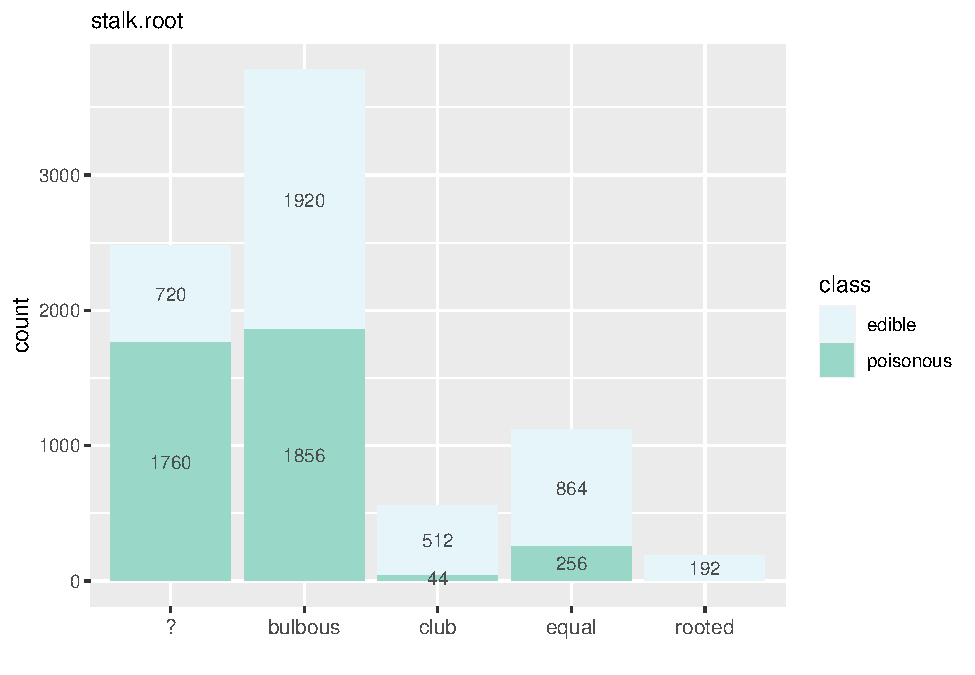
\includegraphics[width=\linewidth]{img/stalkroot-1.pdf}  
      \caption{菌托分布情况}
      \end{subfigure}
      \begin{subfigure}[b]{0.39\textwidth}
        \centering
        % include 2 image
        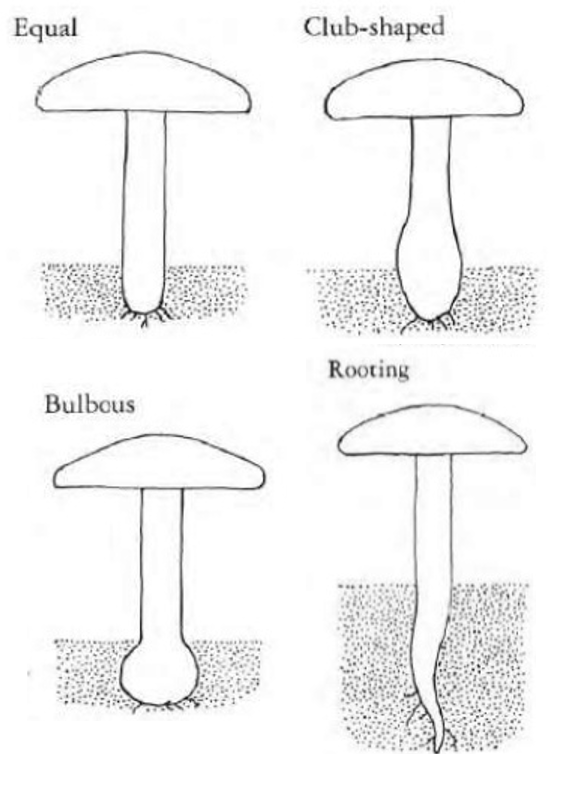
\includegraphics[width=0.8\linewidth,height=2.6in]{img/stalkroot.PNG}  
        \caption{菌托示意图}
        \label{fig:jtsyt}
      \end{subfigure}
      \caption{菌托}
      \label{fig:stalkroot}
   \end{figure}

   \item 环上柄面:\par 有4种取值,分别为fibrous=f,scaly=y,silky=k,smooth=s,
   分布情况如图\ref{fig:ssa}所示,示意图如图\ref{fig:sssy}所示。
   \begin{figure}[hbt]
      \begin{subfigure}[b]{0.49\textwidth}
        \centering
        % include 1 image
        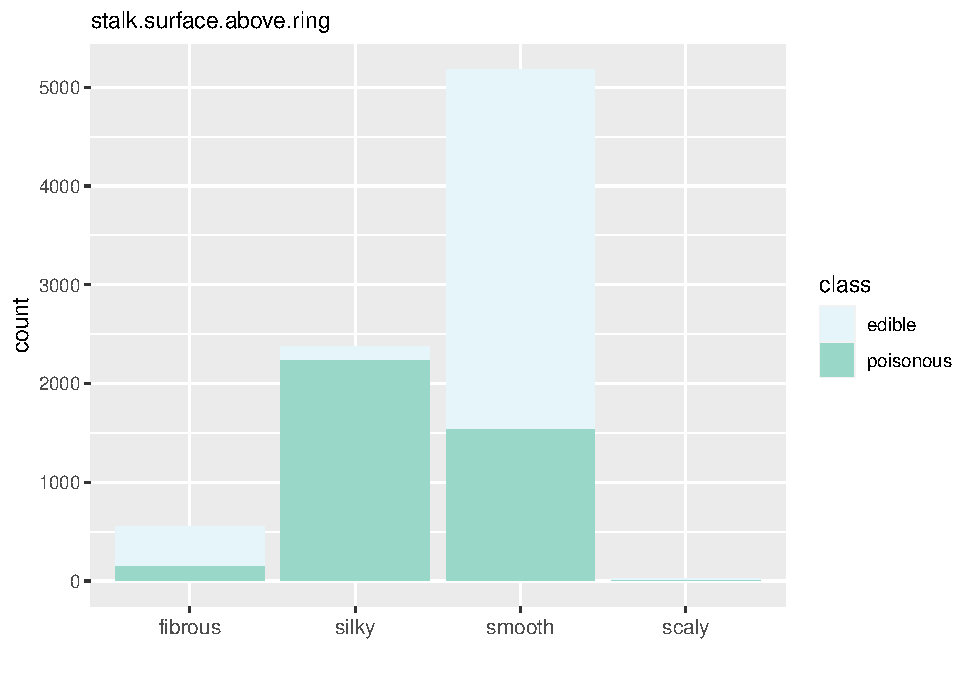
\includegraphics[width=\linewidth]{img/stalksurfaceabovering-1.pdf}  
      \caption{环上柄面分布情况}
      \label{fig:ssa}
      \end{subfigure}
      \begin{subfigure}[b]{0.49\textwidth}
        \centering
        % include 2 image
        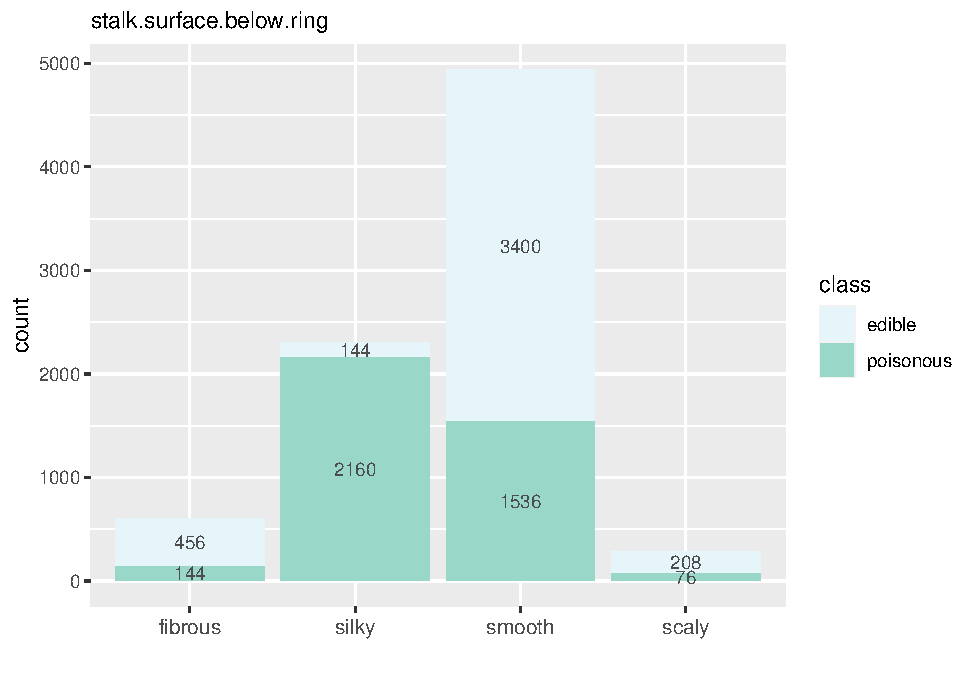
\includegraphics[width=\linewidth]{img/stalksurfacebelowring-1.pdf}  
        \caption{环下柄面分布情况}
        \label{fig:ssb}
      \end{subfigure}
      \caption{柄面}
   \end{figure}

   \begin{figure}[!htbp]
      \centering
      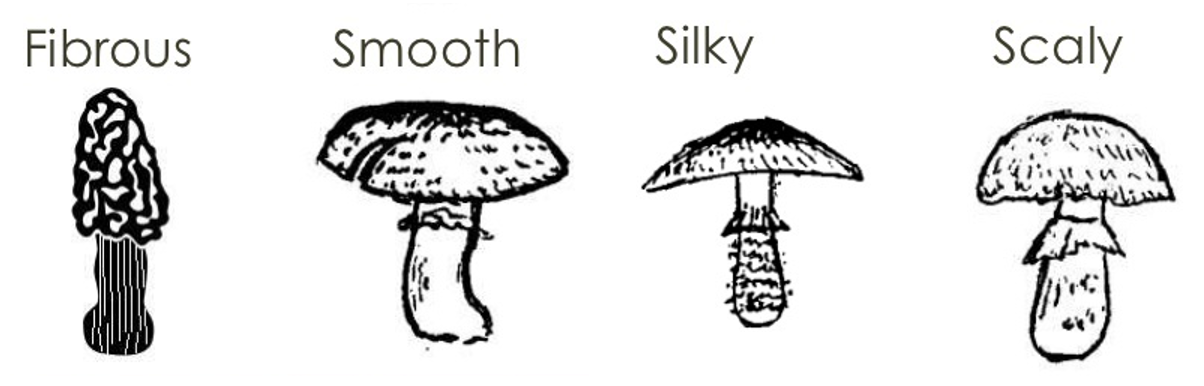
\includegraphics[width=0.7\linewidth]{img/ss.PNG}
      \caption{菌柄形状示意图}
      \label{fig:sssy}
   \end{figure}
   \item 环下柄面:\par 有4种取值,分别为fibrous=f,scaly=y,silky=k,smooth=s,
   分布情况如图\ref{fig:ssb}所示,示意图如图\ref{fig:sssy}所示。
   可以看出环上柄面和环下柄面分布情况大致相同。
   计算发现共有1868个样品环上柄面和环下柄面不同,约占总样品数的23.0\%。

   \item 环上柄色:\par 有9种取值,分别为brown=n,buff=b,cinnamon=c,gray=g,orange=o,
   pink=p,red=e,white=w,yellow=y,如图\ref{fig:sca}所示。
   \begin{figure}[!htbp]
      \begin{subfigure}[b]{0.49\textwidth}
        \centering
        % include 1 image
        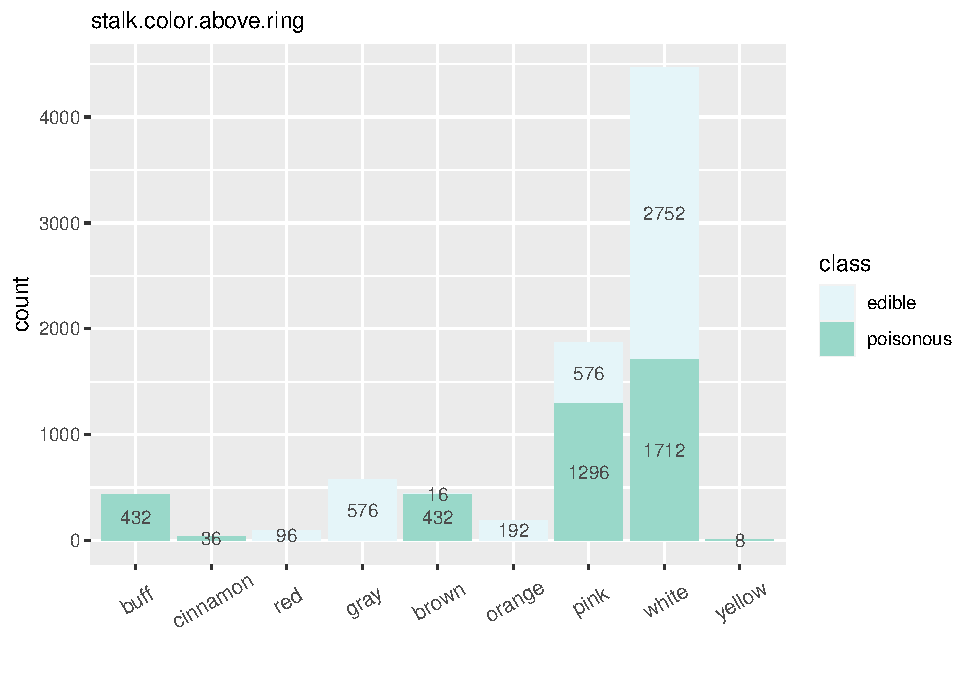
\includegraphics[width=\linewidth]{img/stalkcolorabovering-1.pdf}  
      \caption{环上柄色分布情况}
      \label{fig:sca}
      \end{subfigure}
      \begin{subfigure}[b]{0.49\textwidth}
        \centering
        % include 2 image
        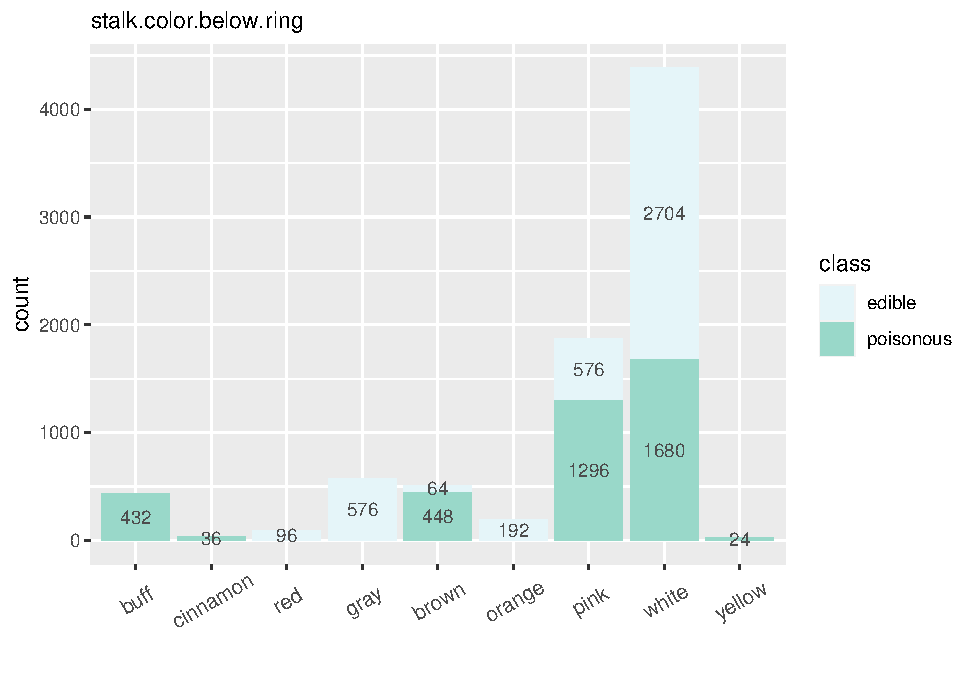
\includegraphics[width=\linewidth]{img/stalkcolorbelowring-1.pdf}  
        \caption{环下柄色分布情况}
        \label{fig:scb}
      \end{subfigure}
      \caption{柄色}
   \end{figure}
   \item 环下柄色:\par 有9种取值,分别为brown=n,buff=b,cinnamon=c,gray=g,orange=o,
   pink=p,red=e,white=w,yellow=y,如图\ref{fig:scb}所示。可以看出环上柄色和
   环下柄色分布情况大致相同。具体地,9种取值中有6种数量上完全相同。猜想环上柄色和
   环下柄色具有很强的相关性。然而计算发现共有3056个样品环上柄色和
   环下柄色不同,约占总样品数的37.6\%。
   
   \item 菌幕类型:\par 只有1种取值,为partial=p。这一特征对分类完全没有帮助,
   因此在章节\ref{sec:delveil}中删除这一特征\footnote{Kaggle上很少有人注意到这类细节。}。

   \item 菌幕颜色:\par 有4种取值,分别为brown=n,orange=o,white=w,yellow=y,
   如图\ref{fig:veilcol}所示。大多数蘑菇菌幕为白色。 菌幕为棕色或橘色的蘑菇均可食用,为黄色的均不可食用。
   \begin{figure}[hbt]
      \begin{subfigure}[b]{0.69\textwidth}
        \centering
        % include 1 image
        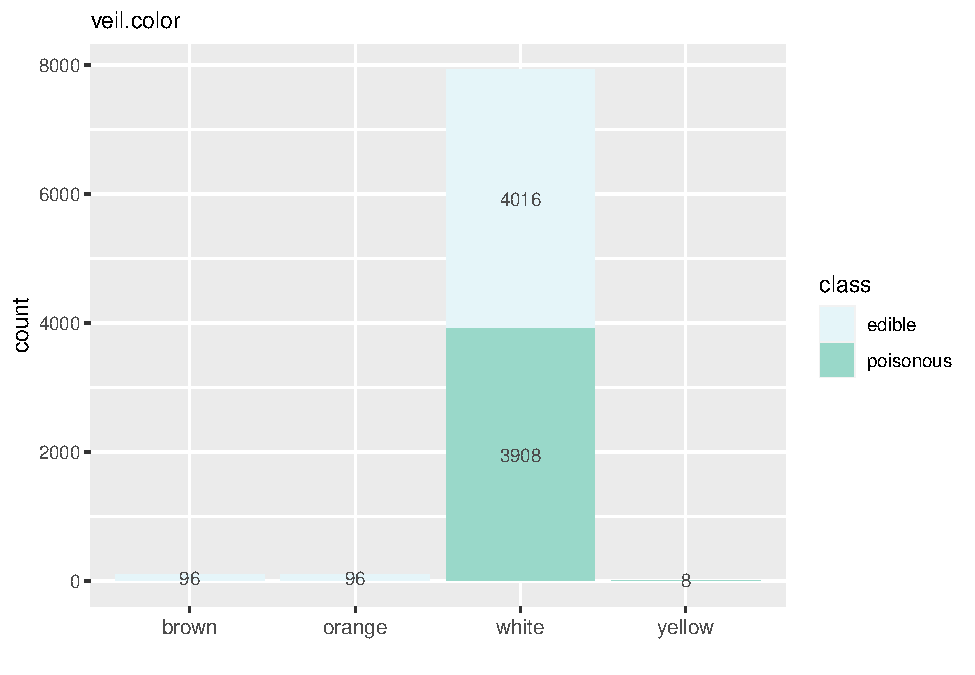
\includegraphics[width=\linewidth]{img/veilcolor-1.pdf}  
      \caption{菌幕颜色分布情况}
      \end{subfigure}
      \begin{subfigure}[b]{0.3\textwidth}
        \centering
        % include 2 image
        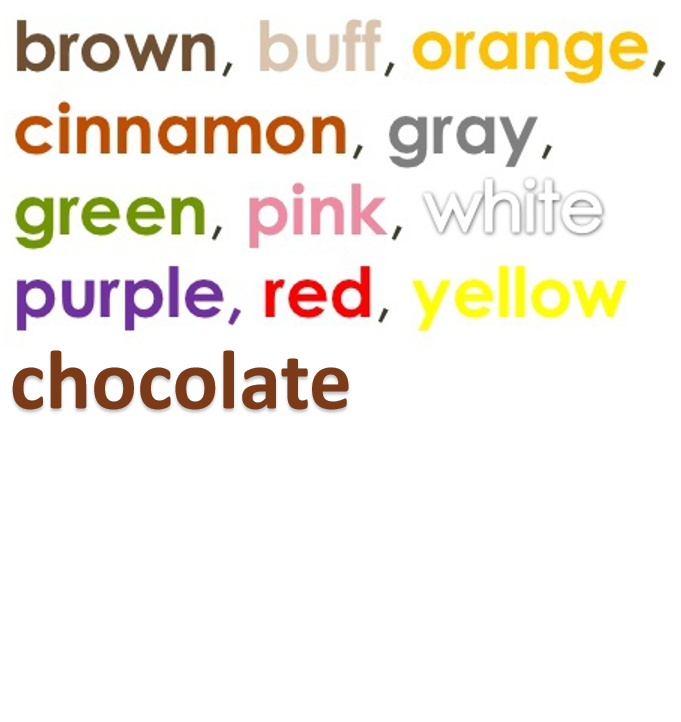
\includegraphics[width=\linewidth]{img/color.PNG}  
        \caption{颜色示意图}
        \label{fig:color}
      \end{subfigure}
      \caption{菌幕颜色}
      \label{fig:veilcol}
   \end{figure}

   \item 菌环数量:\par 有3种取值,分别为无,1,2,如图\ref{fig:rn}所示。
   这份数据集中大部分是有菌环的蘑菇品种,事实上常见的食用蘑菇是没有菌环的。
   可以看出数据集中没有菌环的蘑菇均不可食用。这里可以选择理解为有序因子或无序因子,
   但我认为取无序因子更合适,因为不同菌环数目代表不同类别。
   % \begin{figure}[htb]
   %    \centering
   %    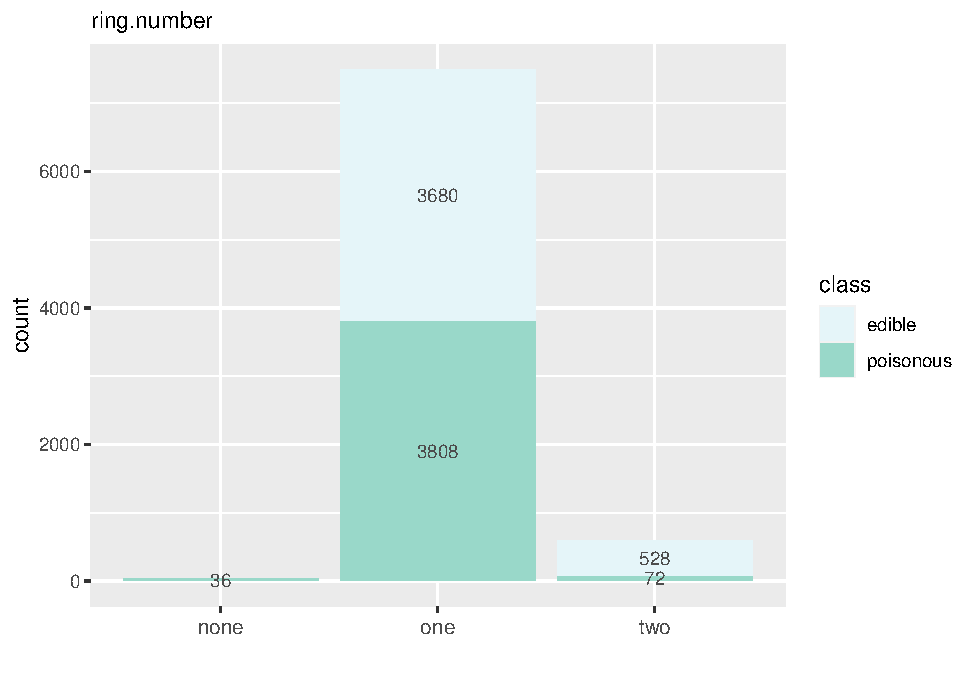
\includegraphics[width=0.6\linewidth]{img/ringnumber-1.pdf}
   %    \caption{菌环数量分布情况}
   %    \label{fig:rn}
   % \end{figure}

   \item 菌环类型:\par 有5种取值,分别为cobwebby=c,evanescent=e,flaring=f,large=l,
   none=n,pendant=p,sheathing=s,zone=z,如图\ref{fig:rt}所示。
   菌环类型为flaring的蘑菇均可食用,有大菌环和没有菌环的均不可食用。
   % \begin{figure}[bth]
   %    \centering
   %    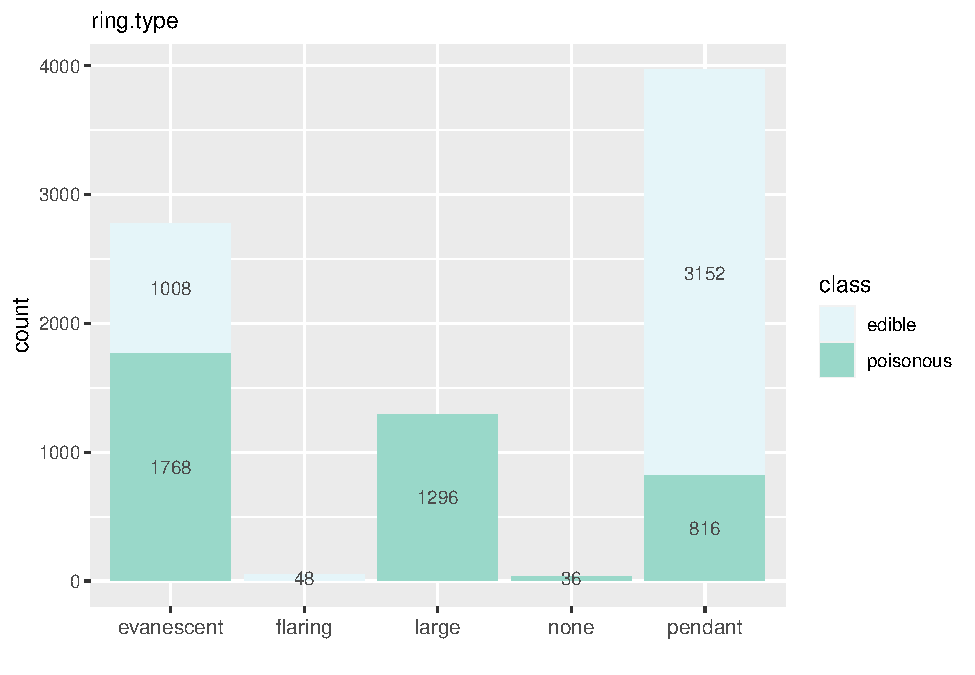
\includegraphics[width=0.6\linewidth]{img/ringtype-1.pdf}  
   %    \caption{菌环类型分布情况}
   %    \label{fig:rt}
   % \end{figure}

   \begin{figure}[bth]
      \begin{subfigure}[b]{0.48\textwidth}
        \centering
        % include 1 image
        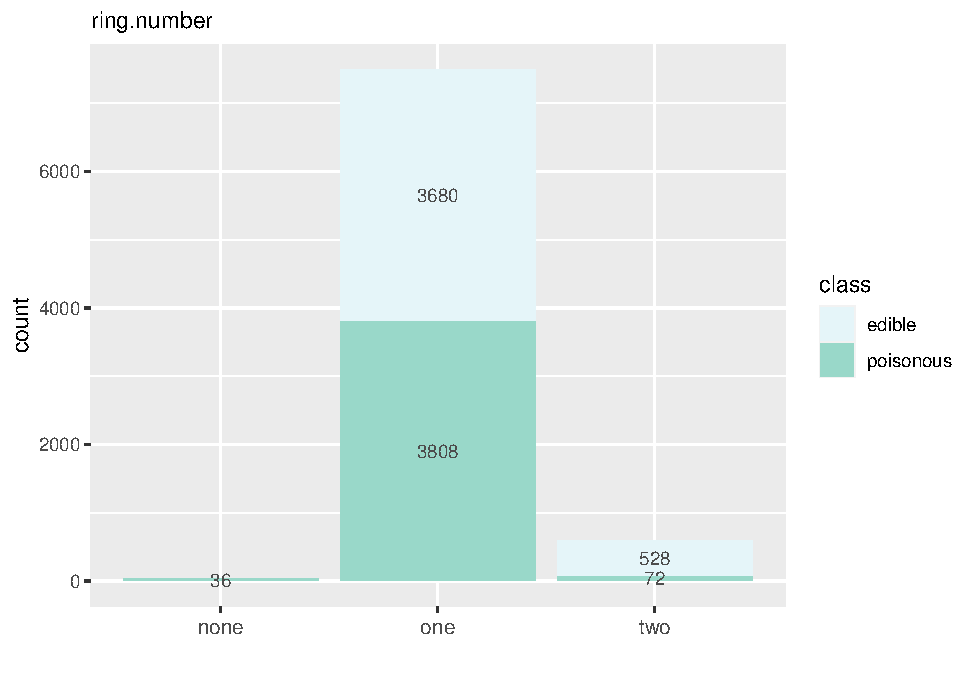
\includegraphics[width=\linewidth]{img/ringnumber-1.pdf}
      \caption{菌环数量分布情况}
      \label{fig:rn}
      \end{subfigure}
      \begin{subfigure}[b]{0.51\textwidth}
        \centering
        % include 2 image
        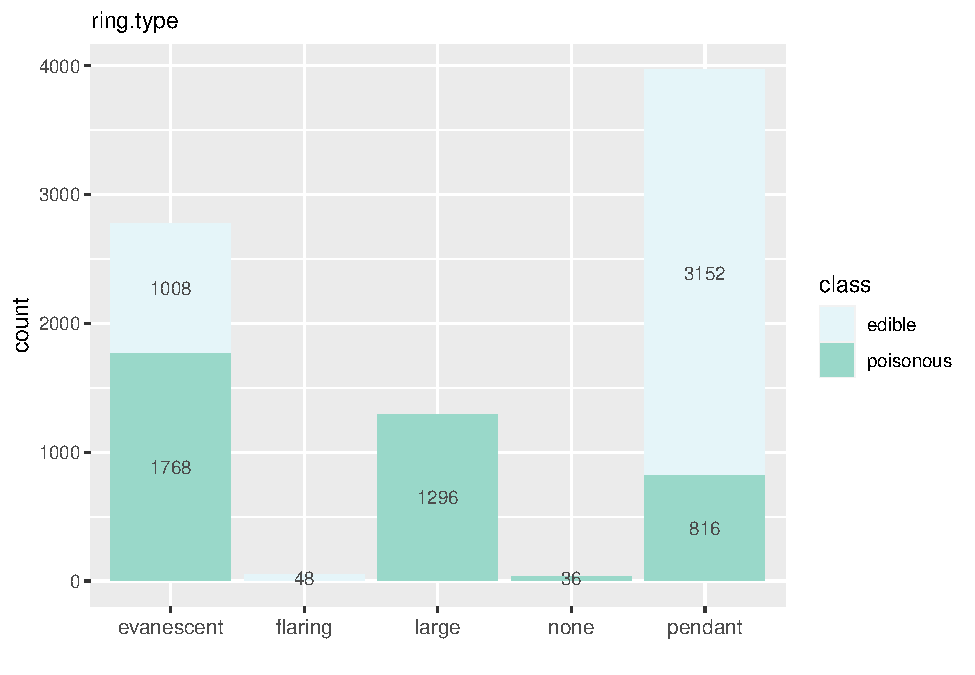
\includegraphics[width=\linewidth]{img/ringtype-1.pdf} 
        \caption{菌环类型分布情况}
        \label{fig:rt}
      \end{subfigure}
      \caption{菌环数量和菌环类型分布情况}
   \end{figure}
   \item 孢子印颜色:\par 有种取值,分别为black=k,brown=n,buff=b,chocolate=h,green=r,
   orange=o,purple=u,white=w,yellow=y,如图\ref{fig:spcol}所示。颜色参见图\ref{fig:color}。
   孢子印颜色为buff、黄色、紫色或橘色的蘑菇均可食用,为黑色或棕色的大多数可以食用,
   为巧克力色和白色的大都不可食用。
   \begin{figure}[bth]
      \begin{subfigure}[b]{0.59\textwidth}
        \centering
        % include 1 image
        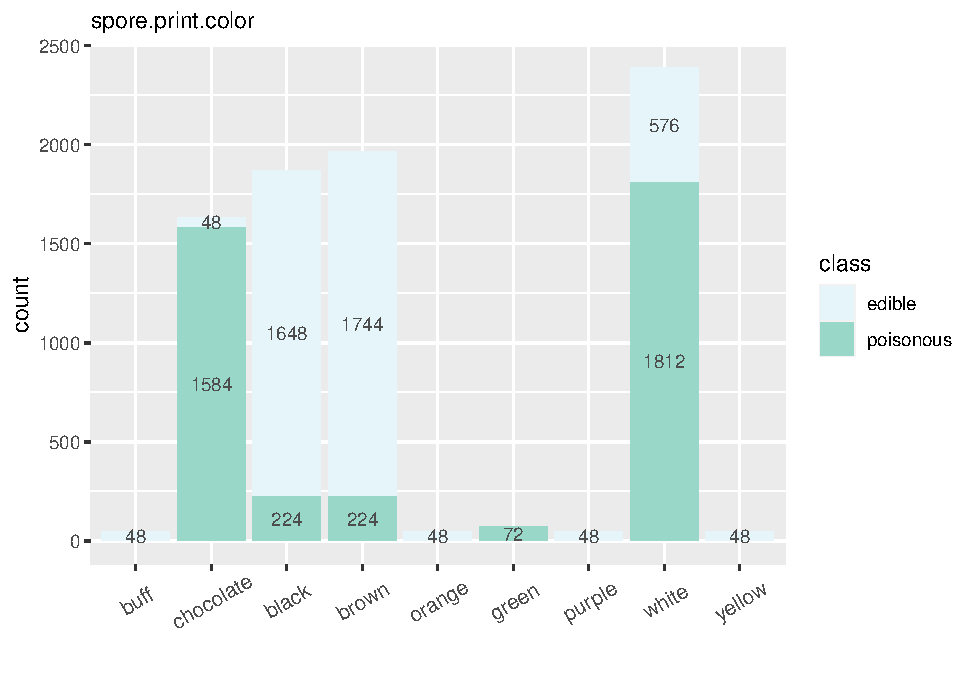
\includegraphics[width=\linewidth]{img/sporeprintcolor-1.pdf}  
      \caption{孢子印颜色分布情况}
      \end{subfigure}
      \begin{subfigure}[b]{0.4\textwidth}
        \centering
        % include 2 image
        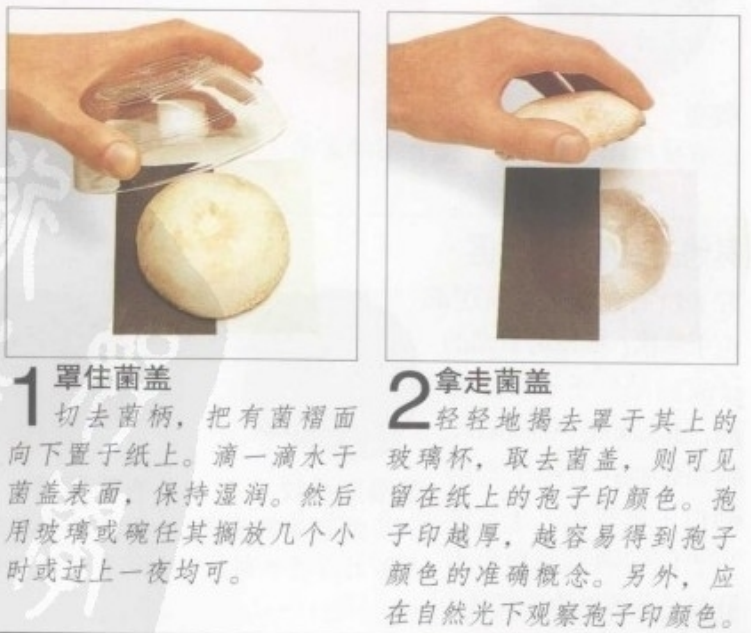
\includegraphics[width=\linewidth,height=2.5in]{img/spprint.PNG}  
        \caption{孢子印获取方式示意图}
      \end{subfigure}
      \caption{孢子印颜色}
      \label{fig:spcol}
   \end{figure}

   \item 生长分布:\par 有6种取值,分别为群生(abundant=a),簇生(clustered=c),叠生(numerous=n),
   散生(scattered=s),丛生(several=v),单生(solitary=y)~\cite{2018tujian},
   如图\ref{fig:szfb}所示。
   生长分布为abundant和numerous的蘑菇均可食用。
   \begin{figure}[bth]
      \begin{subfigure}[t]{0.64\textwidth}
        \centering
        % include 1 image
        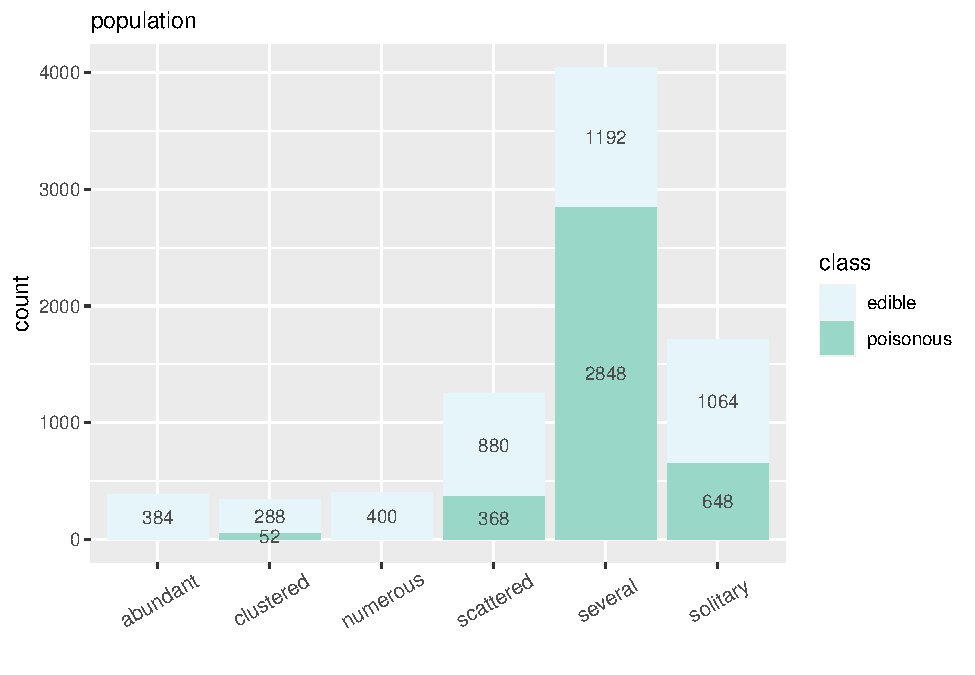
\includegraphics[width=\linewidth]{img/population-1.pdf}   
        \caption{生长分布分布情况}
        \label{fig:szfb}
      \end{subfigure}
      \begin{subfigure}[t]{0.35\textwidth}
        \centering
        % include 2 image
        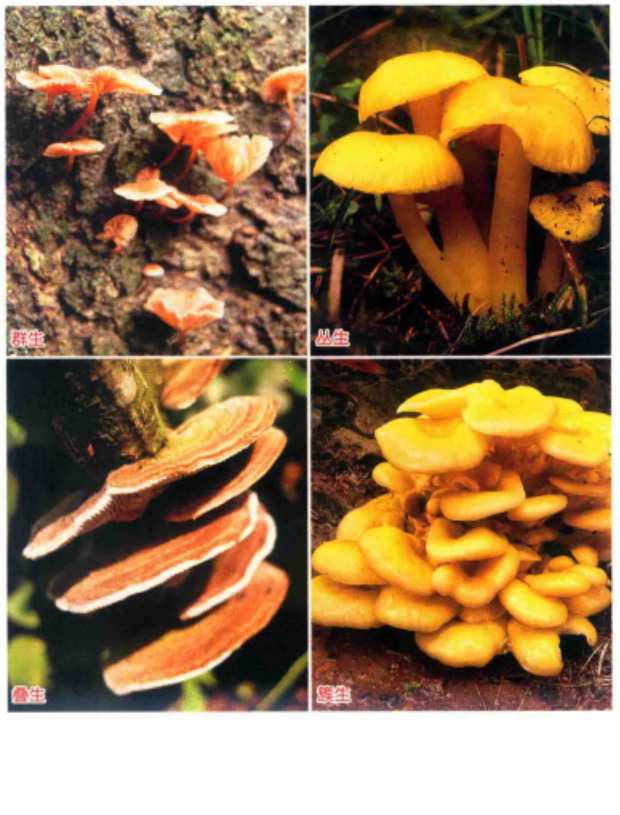
\includegraphics[width=\linewidth,height=2.3in]{img/szfb.PNG}  
        \caption{4种较难区分的生长分布}
      \end{subfigure}
      \caption{生长分布}
   \end{figure}


   \item 生长环境:\par 有7种取值,分别为grasses=g,leaves=l,meadows=m,paths=p,
   urban=u,waste=w,woods=d,如图\ref{fig:szhj}所示。
   生长在有污染的环境的蘑菇均可食用\footnote{感觉违背常识,我专门确认了类别没有标反。},
   生长在路边的蘑菇大多不可食用。
%    \begin{figure}[htb]
%       \begin{subfigure}[b]{0.49\textwidth}
%         \centering
%         % include 1 image
%         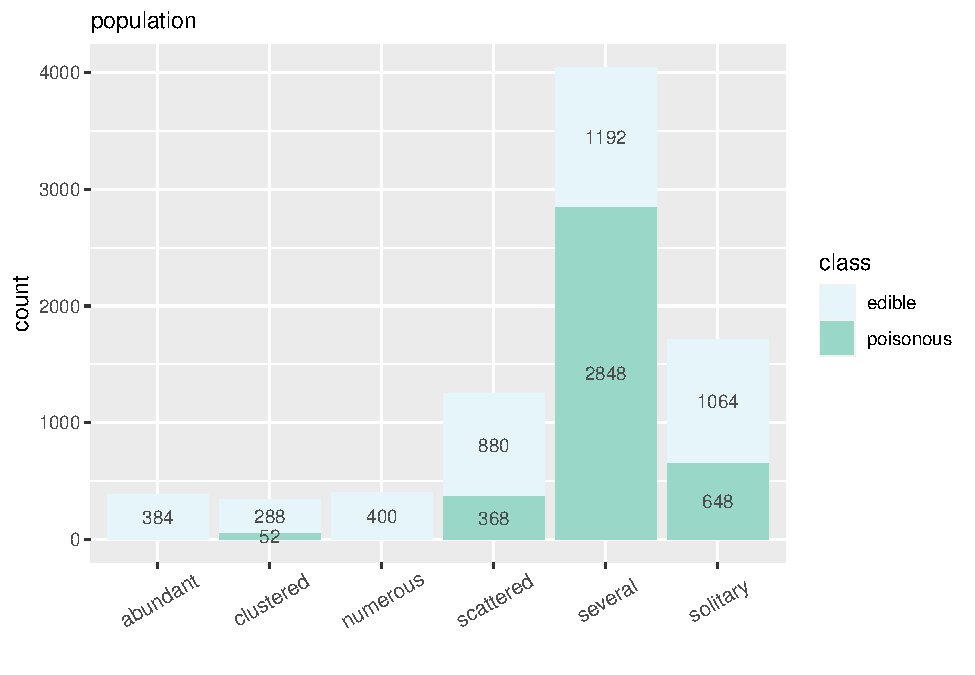
\includegraphics[width=\linewidth]{img/population-1.pdf}  
%       \caption{生长分布分布情况}
%   %    \label{fig:szfb}
%       \end{subfigure}
%       \begin{subfigure}[b]{0.49\textwidth}
%         \centering
%         % include 2 image
%         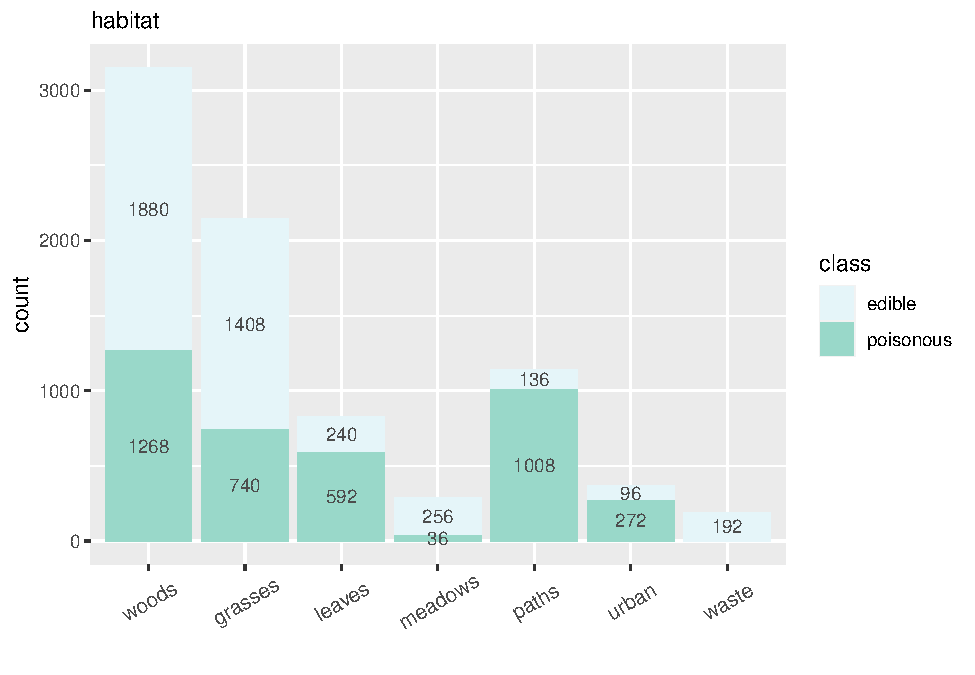
\includegraphics[width=\linewidth]{img/habitat-1.pdf}  
%         \caption{生长环境}
%         \label{fig:szhj}
%       \end{subfigure}
%       \caption{生长分布和生长环境}
%    \end{figure}
\begin{figure}[phtb]
   \centering
   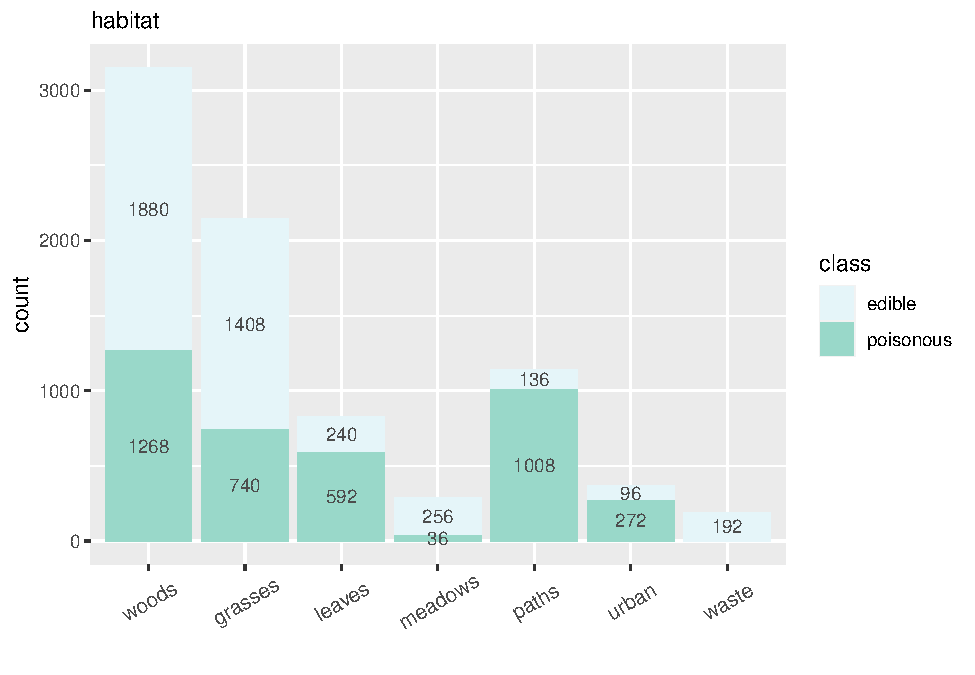
\includegraphics[width=0.8\linewidth]{img/habitat-1.pdf}  
   \caption{生长环境}
   \label{fig:szhj}
\end{figure}
\end{enumerate}

\par 至此,23个特征全部介绍完毕。从上述分析中可以感受到,很多特征都和可以食用或不可以食用有明显的
相关性。这说明利用蘑菇的外形特征判断是否可食用是可行的。
然而,仅根据上面的直方图无法找出准确判断所有蘑菇是否可食用的方法。因此,还需要进一步的数据分析。
\par 此外,注意到表\ref{tab:sjgl}中很多取值并未在数据集中出现,意味着基于此数据集建立的模型可能
不适用于除北美地区 Agaricus 和 Lepiota 科之外的蘑菇食用性鉴别。一些特征的部分取值样本量较少,可能对模型有影响。
\par 接下来,先根据探索性分析对数据进行预处理,再尝试建立判断蘑菇是否可食用的模型。
\par 注:正文未展示的探索性分析见附录\ref{sec:other}。


\section{预处理}
在这一部分中,本文根据探索性分析对数据进行预处理。
读入数据后,删除取值全部相同的特征。之后,利用随机森林计算特征重要性,
进一步确认需要填补缺失值。为避免训练集与测试集之间的数据泄露,在填补缺失值之前
进行训练集与测试集的划分,之后对训练集与测试集分别进行填补。由于数据集中均为因子变量,
为了使用逻辑回归等模型,将因子变量编码为哑变量。
\par 首先,读入附件中的数据集并命名为“mushroom”。
\subsection{删除不必要的特征}\label{sec:delveil}
由于所有样本的veil.type取值相同,这一个特征对分类没有价值,删去这列。
删去后数据保存在data.o中,mushroom可以作为备份数据。
\begin{lstlisting}[style=R]
data.o <-  mushroom
data.o$veil.type <- NULL  
\end{lstlisting}

\subsection{计算变量的重要性}
利用randomForest包的随机森林模型,计算各个变量的MeanDecreaseGini,用于评判
变量的重要性。计算时忽略stalk.root(菌托)缺失的样本。如图\ref{fig:imp}所示,
odor(气味)的重要性远超出其它特征;stalk.root的重要性不该被忽视,因此在\ref{sec:missingdata}
中将对缺失值进行补全。
\begin{figure}[htb]
   \centering
   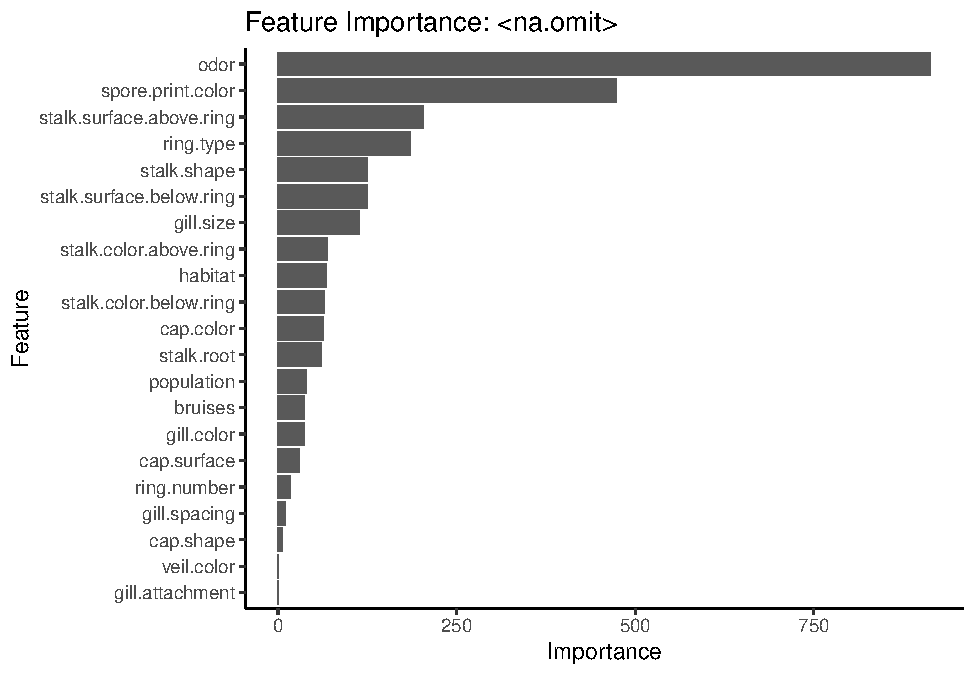
\includegraphics[width=0.9\linewidth]{img/import.omit-1.pdf}
   \caption{变量重要性}
   \label{fig:imp}
\end{figure}

\subsection{划分训练集与测试集}\label{sec:huafen}
如果先进行缺失值填补,训练集的数据情况必将影响测试集。所以,
为避免训练集与测试集之间的数据泄露,本文在填补缺失值之前
进行训练集与测试集的划分。考虑到数据量等因素,划分比例取
训练集:测试集 = 8:2\footnote{与XGBoost划分比例相同}。
划分后,训练集6499个样本,测试集1625个样本。此后,模型训练和参数调整将在训练集中进行,测试集用于计算模型最终的精度。
划分代码如下所示,test.index表示抽取作为测试集的样本序号。
\begin{lstlisting}[style=R]
set.seed(0)
test.index <- sample(1:nrow(data.o), replace = F, size = ceiling(0.2*nrow(data.o))) 
\end{lstlisting}

\subsection{缺失值处理}\label{sec:missingdata}
缺失值从缺失的分布来讲可以分为:
\begin{itemize}
   \item 完全随机缺失(missing completely at random,MCAR):
   数据的缺失是随机的,数据的缺失不依赖于任何不完全变量或完全变量;
   \item 随机缺失(missing at random,MAR):数据的缺失不是完全随机的,即该类数据的缺失依赖于其他完全变量;
   \item 完全非随机缺失(missing not at random,MNAR):数据的缺失依赖于不完全变量自身。
\end{itemize}
缺失值从缺失值的所属属性来讲可以分为:
\begin{itemize}
   \item 单值缺失:如果所有的缺失值都是同一属性;
   \item 任意缺失:缺失值属于不同的属性;
   \item 单调缺失:对于时间序列类的数据,可能存在随着时间的缺失~\cite{queshi}。
\end{itemize}
\par 根据探索性分析第\ref{item:1}条中的分析,认为菌托的缺失属于完全非随机缺失和任意缺失。
根据数据集的特点,选取如下3种填补方法:
\begin{enumerate}
   \item 决策树:使用rpart包的决策树模型预测缺失值;
   \item 多重填补(Multivariate Imputation,MI):
   一种基于重复模拟的处理缺失值方法,处理复杂的缺失值问题最常选用的方法。
   这里采用mice包利用链式方程的多元插补(Multivariate Imputation via Chained Equations,MICE)完成。
   mice()中,缺失值的插补通过Gibbs抽样完成。每个包含缺失值的变量都默认可通过数据集中的其他变量预测得来, 
   于是这些预测方程便可用来预测缺失数据的有效值 ~\cite{ria}。mice()填补过程示意图如图\ref{fig:mice}所示。
   \begin{figure}[!htbp]
      \centering
      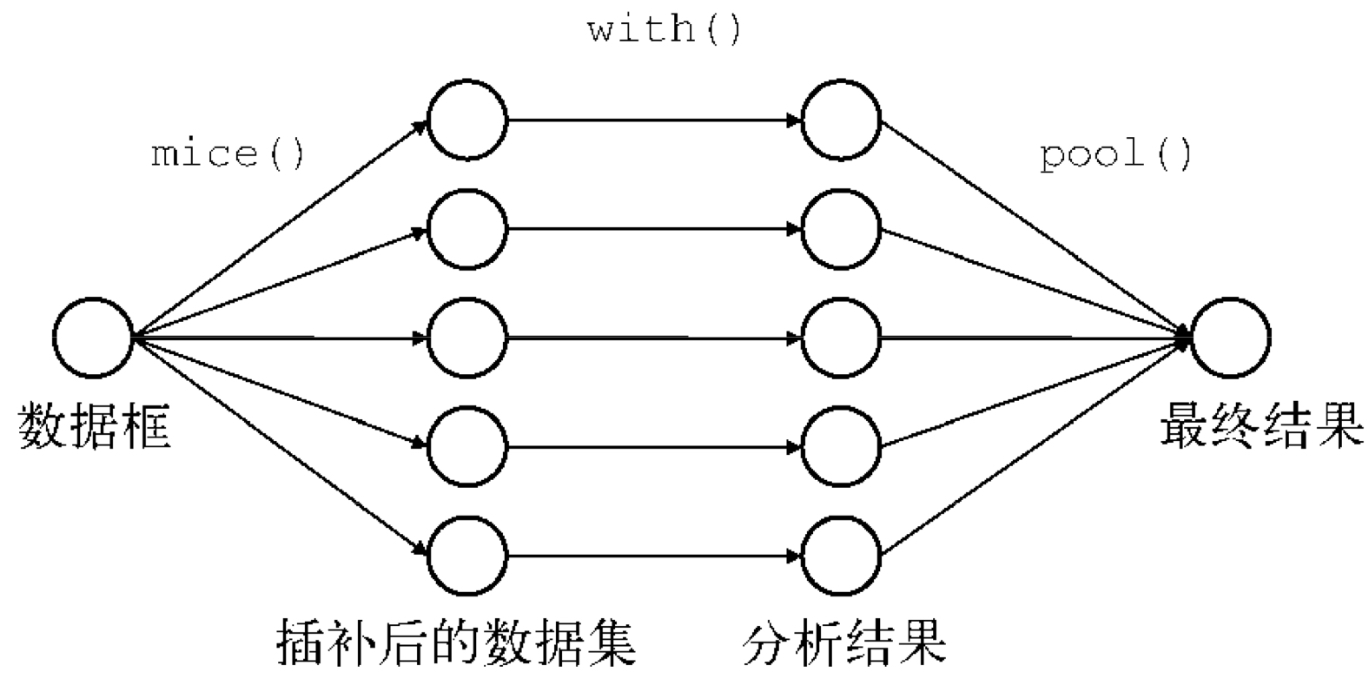
\includegraphics[width=0.7\linewidth]{img/mice.jpg}
      \caption{通过MICE包应用多重插补的步骤:函数mice()首先从一个包含缺失数据的数据框开始,然后
      返回一个包含多个(默认为5个) 完整数据集的对象。 每个完整数据集都是通过对原
      始数据框中的缺失数据进行插补而生成的。 由于插补有随机的成分,因此每个完整数
      据集都略有不同。然后,with()函数可依次对每个完整数据集应用统计模型(如线性模
      型或广义线性模型) 。最后,pool()函数将这些单独的分析结果整合为一组结果。最终模
      型的标准误和p值都将准确地反映出由于缺失值和多重插补而产生的不确定性。}
      \label{fig:mice}
   \end{figure}

   \item k近邻(k Nearest Neighbors,kNN):使用VIM包的kNN()预测缺失值。
\end{enumerate}
\par 为选取最适合数据集的填补方法,将随机地在无缺失样本中人为制造缺失值,再分别用上述3种方法预测,以此判断填补方法的效果。
具体步骤如下:
\begin{enumerate}
   \item 取出不含缺失值的样本,同时把目标变量class排除在外
   \footnote{删去目标变量是有必要的,因为后续需要用菌托来预测蘑菇是不是可食用。};
   \item 将上述样本按7:3划分为训练集和测试集。选取这个比例的原因是:原数据中缺失比例约为30\%;
   \item 分别用3种方法在训练集上训练\footnote{这里kNN参数k的确定最好使用交叉检验};
   \item 分别用3种方法在测试集上测试,并记录结果。
\end{enumerate}
\par 结果如表\ref{tab:tianbu}所示。其中,kNN的k值为3。可以看出kNN效果最好,在测试集上全部预测正确。
同时其它两个方法效果也很好。
\begin{table}[!htbp]
   \centering
   \caption{3种方法的填补准确率}
   \label{tab:tianbu}
   \setlength{\tabcolsep}{7mm}{
   \begin{tabular}{cccc} 
   \toprule
   方法  & kNN & mice   & rpart   \\
   \midrule
   准确率 & 1  & 0.9994 & 0.9947  \\
   \bottomrule
   \end{tabular}}
\end{table}
最终选用的方法是kNN(k = 3)。使用KNN在\ref{sec:huafen}中确定的训练集和测试集上进行填补。
选用kNN不仅是因为这个方法效果最好,还因为它满足模型在进化论上的意义。理论上其它特征相似的
蘑菇应该有相似的菌托。同时k选取3也允许这一情况的存在:两种蘑菇除了菌托不同,其它特征相同。
\begin{lstlisting}[style=R]
data.o$stalk.root[na.index] = NA
data.o$stalk.root = factor(data.o$stalk.root)
train.x = kNN(data.o[-test.index, -1], variable = 'stalk.root', k = 3)
train.x$stalk.root_imp = NULL
train.y = data.o[-test.index, 1]
train.data = train.x
train.data$class = train.y
test.x = kNN(data.o[test.index, -1], variable = 'stalk.root', k = 3)
test.x$stalk.root_imp = NULL
test.y = data.o[test.index, 1]
test.data = test.x
test.data$class = test.y
\end{lstlisting}
\par 填补后stalk.root分布变化如图\ref{fig:afterimp}所示。
填补主要集中在bulbous 与equal,这说明探索性分析\ref{item:1} 中的猜测应该是正确的,
缺失值的出现很可能是因为这两类菌托难以分辨。
\begin{figure}[htb]
   \centering
   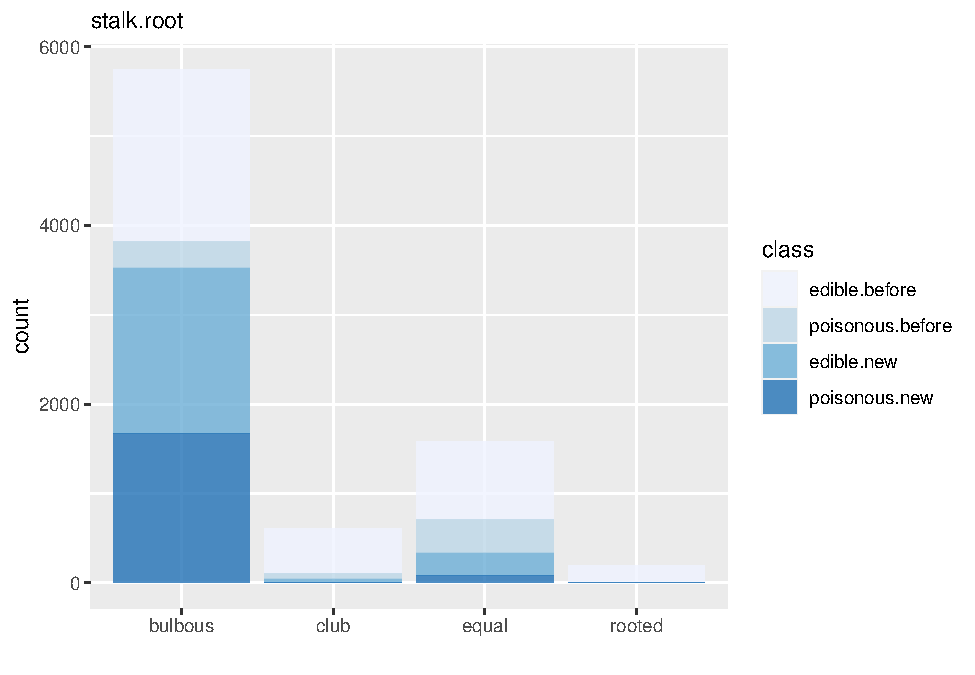
\includegraphics[width=0.8\linewidth]{img/afterimp-1.pdf}
   \caption{填补前后菌托分布情况}
   \label{fig:afterimp}
\end{figure}


\subsection{编码为哑变量}
填补完成后,将因子变量编码为哑变量。注意到由于个别特征取值的数量过少,可能全部被分到训练集中,
导致测试集中不存在该取值。编码成哑变量会使得训练集和测试集变量数目不同,使得模型无法运行。
因此需先检查是否存在上述取值,编码后手动调整,为测试集添加变量
\footnote{我有考虑过先编码哑变量,再划分训练集和测试集,最后进行填补。这样就不会出现这个问题。
但是编码成哑变量后很难填补,所以最终决定最后编码哑变量。}。
\par 使用dummies包编码哑变量代码如下所示。
\begin{lstlisting}[style=R]
library(dummies)
train.xd = dummy.data.frame(train.x, sep = ".")
train.xd = train.xd[, order(colnames(train.xd))]
train.yd = as.numeric(train.y) - 1
train.d = train.xd
train.d$class = train.yd

test.xd = dummy.data.frame(test.x, sep = ".")
test.xd$cap.surface.g = 0
test.xd = test.xd[, order(colnames(test.xd))]
test.yd = as.numeric(test.y) - 1
test.d = test.xd
test.d$class = test.yd
\end{lstlisting}
\par 最终数据集变为:
\begin{lstlisting}[style=R]
  bruises cap.color.b cap.color.c cap.color.e cap.color.g  ...
1    TRUE           0           0           0           0  ...
2    TRUE           0           0           0           0  ...
3    TRUE           0           0           0           0  ...
4    TRUE           0           0           0           0  ...
5   FALSE           0           0           0           1  ...
6    TRUE           0           0           0           0  ...
\end{lstlisting}
即由23个变量,扩展为114个可以由\{0,1\}编码的变量。
\par 编码后可以计算变量之间相关性\footnote{Kaggle上很多教程默认变量为有序因子
,然后计算相关性。这样显然不对。},如图\ref{fig:cor}所示。右边第一列是类别变量,
和几乎所有哑变量都有较强的相关性。部分变量之间相关性较强,提示在回归时可能有多重共线性的问题。
\begin{figure}[htb]
   \centering
   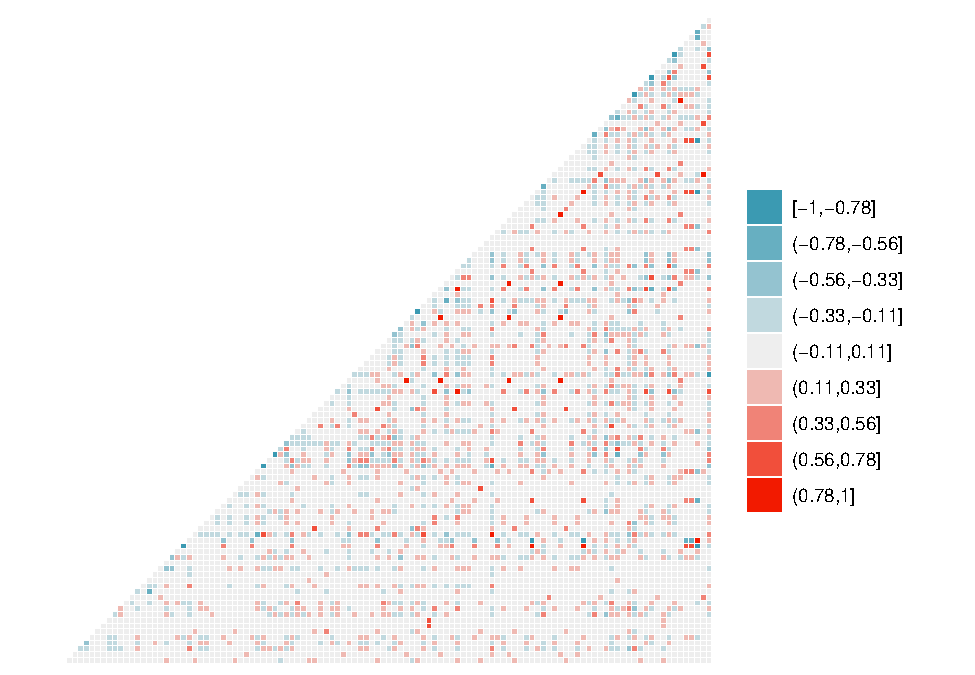
\includegraphics[width=\textwidth]{img/cor-1.pdf}
   \caption{114个变量的相关性}
   \label{fig:cor}
\end{figure}


\section{数据分析}
这一部分将使用降维(主成分回归、线性判别分析、LASSO回归、逐步回归)、
树(决策树、随机森林、XGBoost)和其它可以使用的方法(kNN、SVM、神经网络、JPip、PART)
对蘑菇数据集进行建模分析。
\subsection{降维}
根据图\ref{fig:cor}的分析,考虑到编码为哑变量的数据集可能存在多重共线性,同时114个自变量如果
直接进行逻辑回归会造成维度爆炸。所有在进行回归之前,要么选择变量,要么尝试用较低的维度表示高维数据。
可选的方法有主成分回归、线性判别分析、LASSO回归和逐步回归。这几种方法都需要用哑变量编码的数据。
\begin{enumerate}
   \item 主成分回归:\par 参考《应用多元统计分析》进行主成分回归。
   首先将114个自变量用几个主成分表示,进行逻辑回归,再利用PCA的旋转矩阵将回归系数转换成
   原始变量的回归系数,由此建立逻辑回归模型~\cite{ghx}。选取主成分为4,5,6,7
   \footnote{原始变量间多重共线性并不强,并且这里的主成分也找不到特殊的含义。
   同时,20个PCs才解释80\%的方差,31个PCs才解释90\%的方差。说明PCR不是合适的模型。}
   利用pROC包绘制ROC曲线并计算AUC,如图\ref{fig:pcrroc}所示。AUC随着PCs数量的增加而增加。
   当PCs=7时,在测试集上分类正确率最高为93.85\% 。
   \begin{figure}[htb]
      \centering
      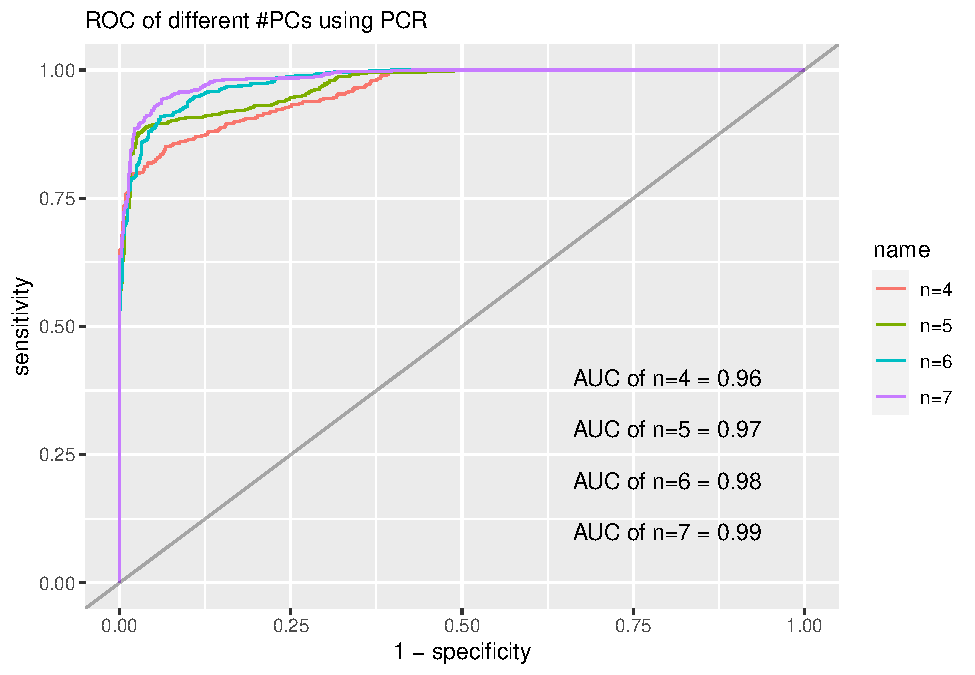
\includegraphics[width=0.8\textwidth]{img/pcr.roc-1.pdf}
      \caption{PCR的ROC曲线及AUC}
      \label{fig:pcrroc}
   \end{figure}
   \item 线性判别分析:使用MASS包的lda(),在测试集上分类正确率为99.88\%。
   \item LASSO回归:\par LASSO回归在普通线性回归上增加了约束
   $\sum_{j=1}^{r}\left|\beta_{j}\right| \leq c$ 。问题的正则形式是寻找$\boldsymbol{\beta}$
   最小化
   $$\phi(\boldsymbol{\beta})=(\mathcal{Y}-\mathcal{X} 
   \boldsymbol{\beta})^{\tau}(\mathcal{Y}-\mathcal{X}
    \boldsymbol{\beta})+\lambda \sum_{j=1}^{r}\left|\beta_{j}\right|.~\cite{jiaocai}$$
    使用glmnet包的cv.glmnet()在测试集上通过交叉验证选择合适的参数。将合适的参数代入glmnet()
    获得最终的模型,模型在测试集上分类正确率为100\%\footnote{LASSO的优势在于可以变量选择。
    它在114个自变量(哑变量)中选择了28个用于回归。选出的28个变量涉及到原有22个自变量中的21个。}。
   \item 逐步回归:\par 使用step()对逻辑回归模型进行后向逐步回归\footnote{运行了将近2h。},
   在测试集上分类正确率为100\% 。
\end{enumerate}

\subsection{树}
使用决策树、随机森林等模型的优势在于不需要使用哑变量编码,对于因子型数据操作方便。
同时,决策树模型可以给出一个明确且可以在现实中推广的判别模型。而随机森林和XGBoost都可以给出变量的
重要性,由此可知哪些特征对判断蘑菇是否可食用最有帮助。接下来将使用
决策树、随机森林和XGBoost建立模型。
\begin{enumerate}
   \item CART决策树:\par  使用rpart包的rpart()建立基于CART算法的决策树模型,调整cp值使树尽可能生长,得到如图
   \ref{fig:cart}所示的决策树\footnote{决策树左下角6个错误分类的样品情况比较复杂,为避免过拟合,树不继续生长}
   ,选择的特征为:odor、spore.print.color、
   stalk.color.below.ring和stalk.surface.above.ring 。在测试集上正确率为99.88\%。
   \begin{figure}[htb]
      \centering
      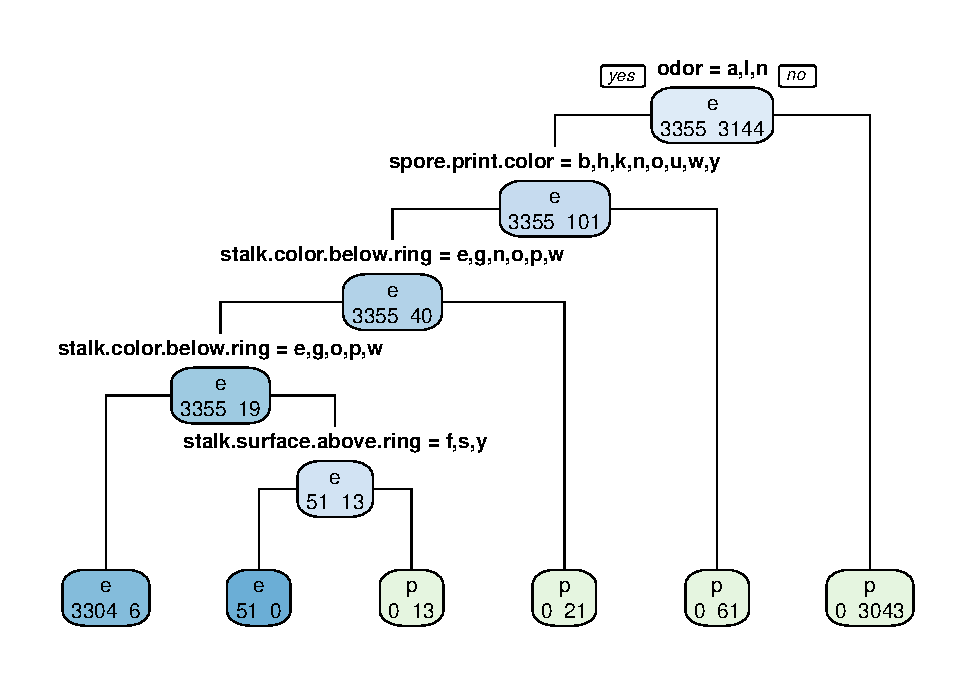
\includegraphics[width=0.85\textwidth]{img/dt-1.pdf}
      \caption{CART决策树}
      \label{fig:cart}
   \end{figure}
   \item C4.5决策树:\par  相对于CART算法使用结点不纯度选择最佳的分裂特征,C4.5算法选择信息增益比$g_R(D,A)$
   完成这一过程。
   为定义信息增益比,首先定义信息增益:
   \begin{definition}
      \textbf{(信息增益)}特征$A$对训练数据集$D$的信息增益$g(D,A)$,定义为集合 $D$的经验熵 $H(D)$与特征$A$给定条件
       $D$下的经验条件熵 $D(D|A)$之差,即 $$g(D, A)=H(D)-H(D|A).$$
   \end{definition}
   再定义信息增益比:
   \begin{definition}
      \textbf{(信息增益比)}特征$A$对训练数据集$D$的信息增益比$g_R(D,A)$定义
      为其信息增益$g(D,A)$与训练数据集 $D$关于特征$A$的值的熵$H_A(D)$之比,即
      $$g_{R}(D, A)=\frac{g(D, A)}{H_{A}(D)}$$
      其中,$H_{A}(D)=-\sum_{i=1}^{n} \frac{\left|D_{i}\right|}{|D|} \log _{2} \frac{\left|D_{i}\right|}{|D|}$
      ,$n$ 是特征$A$取值的个数~\cite{lihang}。
   \end{definition}
   \par 同时,C4.5在构造树的过程中剪枝且可以处理缺失值~\cite{c45}。使用RWeka包的J48()
   绘制的决策树如下所示。选择的特征为:odor、spore.print.color、gill.size、
   gill.spacing和population。前两个特征和CART决策树选择的一致。
   模型在测试集上正确率为100\%。使用含有缺失值的数据(即未经过补全,且缺失值设置为NA的数据)
   时,测试集上正确率为85.29\%。
\begin{lstlisting}
   J48 pruned tree
   ------------------
   
   odor = a: e (307.0)
   odor = c: p (154.0)
   odor = f: p (1741.0)
   odor = l: e (316.0)
   odor = m: p (33.0)
   odor = n
   |   spore.print.color = b: e (37.0)
   |   spore.print.color = h: e (39.0)
   |   spore.print.color = k: e (1053.0)
   |   spore.print.color = n: e (1081.0)
   |   spore.print.color = o: e (34.0)
   |   spore.print.color = r: p (61.0)
   |   spore.print.color = u: e (0.0)
   |   spore.print.color = w
   |   |   gill.size = b: e (405.0)
   |   |   gill.size = n
   |   |   |   gill.spacing = c: p (28.0)
   |   |   |   gill.spacing = w
   |   |   |   |   population = a: e (0.0)
   |   |   |   |   population = c: p (12.0)
   |   |   |   |   population = n: e (0.0)
   |   |   |   |   population = s: e (0.0)
   |   |   |   |   population = v: e (39.0)
   |   |   |   |   population = y: e (0.0)
   |   spore.print.color = y: e (44.0)
   odor = p: p (198.0)
   odor = s: p (471.0)
   odor = y: p (446.0)
   
   Number of Leaves  : 	24
   
   Size of the tree : 	29
\end{lstlisting}

   \item C5.0决策树:\par  C5.0比C4.5更快更高效,同时采用Boosting方式提高模型准确率。使用C50包的C5.0()
   绘制的决策树如图\ref{fig:c50}所示,变量重要性如图\ref{c50imp}所示,选择的特征为:odor、spore.print.color、cap.surface、stalk.color.below.ring和stalk.surface.above.ring,和CART相同。
   其在测试集上正确率为99.88\%。使用含有缺失值的数据时,测试集上正确率为99.88\%。
   相对于C4.5算法,C5.0在含缺失值数据上有很好的表现。注意到C4.5和C5.0都是多叉树。
   \begin{figure}[htb]
      \centering
      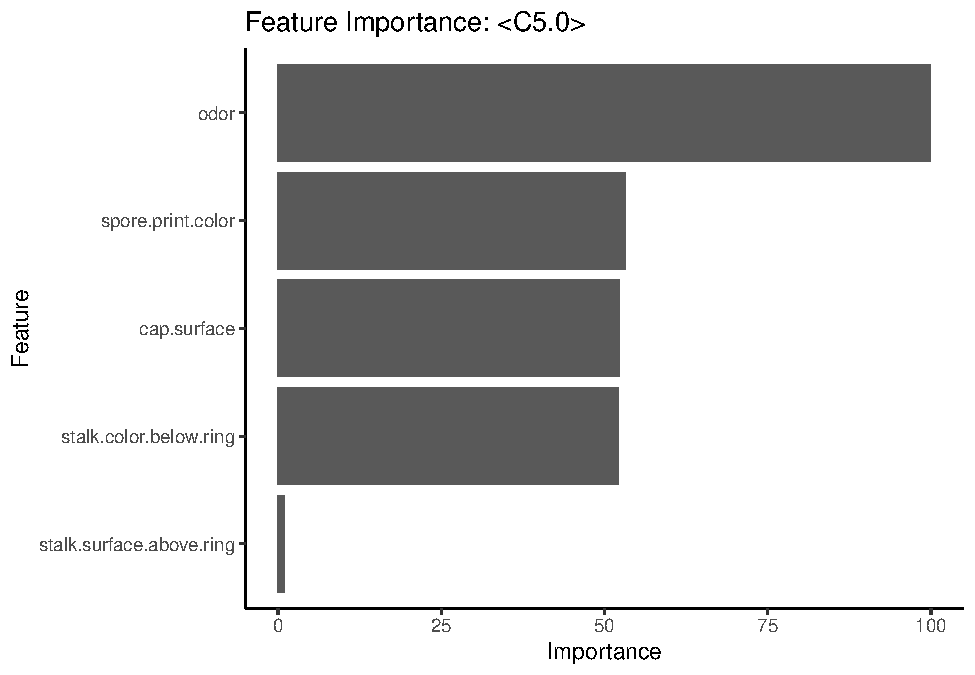
\includegraphics[width=0.6\textwidth]{img/c50imp-1.pdf}
      \caption{C5.0变量重要性}
      \label{fig:c50imp}
   \end{figure} 
   \begin{figure}[hbt]
      \centering
      \includegraphics[width=\textwidth]{img/c50.pdf}
      \caption{C5.0决策树}
      \label{fig:c50}
   \end{figure} 
   \item 随机森林:\par  使用randomForest包的randomForest(),测试集特征的重要性如图\ref{fig:rfmodelimp}所示。  
   重要性较高的特征有:odor、spore.print.color、gill.color、gill.size、stalk.color.below.ring和stalk.surface.above.ring。
   无论是否含有缺失值,在测试集上正确率均为100\%。
   \begin{figure}[hbt]
      \centering
      \includegraphics[width=0.9\textwidth]{img/rfmodelimp-1.pdf}
      \caption{随机森林特征重要性}
      \label{fig:rfmodelimp}
   \end{figure}
   \item XGBoost:\footnote{我原本以为这一部分会相对轻松,因为Mushroom是XGBoost的示例数据集,但还是因为数据
   格式等问题,调试很久才做出来。}
   \par  XGBoost(eXtremeGradient Boosting)将多个CART模型集成在一起,
   形成一个很强的分类器。通过不断地添加树,不断地进行特征分裂来生长一棵树。测试样本在每棵树中
   都会落到一个对应于特定分数的叶子节点,将分数相加就是预测值。
   \par XGBoost的目标函数为
   $$\begin{array}{l}
      \mathcal{L}(\phi)=\sum_{i} l\left(\hat{y}_{i}, y_{i}\right)+\sum_{k} \Omega\left(f_{k}\right) \\
      \text { where } \Omega(f)=\gamma T+\frac{1}{2} \lambda\|w\|^{2}.
      \end{array}$$
      其中,$l\left(\hat{y}_{i}, y_{i}\right)$为可微凸损失函数,
      用于测量预测和目标之间的差异;$T$ 表示叶子节点数;$w$表示叶子节点权重。
  \par 利用泰勒展开可以近似得到第t次迭代的目标函数
  $$\tilde{\mathcal{L}}^{(t)}=\sum_{i=1}^{n}\left[g_{i} f_{t}\left(\mathbf{x}_{i}\right)+
  \frac{1}{2} h_{i} f_{t}^{2}\left(\mathbf{x}_{i}\right)\right]+\Omega\left(f_{t}\right)$$
   其中,$g_{i}=\partial_{\hat{y}(t-1)} l\left(y_{i}, \hat{y}^{(t-1)}\right)$ ,
    $h_{i}=\partial_{\hat{v}(t-1)}^{2} l\left(y_{i}, \hat{y}^{(t-1)}\right)$。
      对于给定的实例,计算叶子节点权重的公式为
      $$w_{j}^{*}=-\frac{\sum_{i \in I_{j}} g_{i}}{\sum_{i \in I_{j}} h_{i}+\lambda},$$
      目标函数可以化简为
      $$\tilde{\mathcal{L}}^{(t)}(q)=-\frac{1}{2} \sum_{j=1}^{T} \frac{\left(
         \sum_{i \in I_{j}} g_{i}\right)^{2}}{\sum_{i \in I_{j}} h_{i}+\lambda}+\gamma T,$$
      结点分裂可通过计算
      $$\mathcal{L}_{s p l i t}=\frac{1}{2}\left[\frac{\left(\sum_{i \in I_{L}} 
      g_{i}\right)^{2}}{\sum_{i \in I_{L}} h_{i}+\lambda}+\frac{\left(\sum_{i \in I_{R}}
       g_{i}\right)^{2}}{\sum_{i \in I_{R}} h_{i}+\lambda}-
      \frac{\left(\sum_{i \in I} g_{i}\right)^{2}}{\sum_{i \in I} h_{i}+\lambda}\right]-\gamma$$
      选择。
     \par  XGBoost还提出了两种防止过拟合的方法:Shrinkage 和 Column(Feature) Subsampling。
      Shrinkage方法是在每次迭代中对树的每个叶子结点的分数乘上一个缩减权重η,类似随即优化中的学习率。
      Column Subsampling 也在随机森林中使用~\cite{xgb}。
   \par 使用xgboost包中xgb.cv()先在训练集上通过5折交叉检验寻找最佳参数,之后使用该参数用xgboost()建立模型,
   并在测试集上进行预测,得到正确率为99.63\%,绘制的变量重要性如图\ref{fig:xgb}所示。
   \begin{figure}[hbt]
      \centering
      \includegraphics[width=0.7\textwidth]{img/xgb-1.pdf}
      \caption{XGBoost特征重要性}
      \label{fig:xgb}
   \end{figure}
\end{enumerate}
\par 综合上述讨论,基于树的模型表现都相当不错。几种算法都认为odor(气味)是最重要的指标,除了
XGBoost之外的4种方法认为spore.print.color(孢子印颜色)是第二重要的指标。

\subsection{其它}
这一部分讨论其它可以使用的方法,包括kNN、SVM、NN和规则学习算法RIPPER与PART。
\begin{enumerate}
   \item kNN:\par 使用class包的knn()选择k=1,在测试集上正确率为100\%。
   \item SVM:\par 使用e1071包的svm()\footnote{SVM参数没有用tune选择,因为这个函数对3*5个参数情况运行了
   超过2h还没有结果。并且默认参数在训练集上正确率为99.98\% 。},在测试集上正确率为100\%。
   \item NN~\cite{mlwr}:\par 神经网络(Neural Network,NN)的设计模拟了生物体神经元间信号传递
   的过程。  
   图\ref{fig:nn1}为一个单一的神经元模型。有向网络图定义
了树突接收的输入信号(变量x)和输出信号(变量y)
之间的关系。与生物神经元一样,每一个树突的信号都
根据其重要性被加权($W_i$),输入信号由细胞体求和,然后该信号根据一
个用f表示的激活函数( Activation Function)来传递。
\begin{figure}[htb]
   \centering
   \includegraphics[width=0.4\textwidth]{img/nn1.PNG}
   \caption{神经元模型示意图}
   \label{fig:nn1}
\end{figure}
   神经网络像搭积木一样使用神经元来构造复杂的模型,可由以下3种特征定义:
   \begin{itemize}
      \item \textbf{ 激活函数:}将高维输入信号转为一维输出信号,最常用的是S形激活函数(Sigmoid Activation function),如图\ref{fig:nns}所示;
      \item \textbf{网络拓扑(Network Topology )或结构(Architecture):}
      描述模型中神经元的数量、层数和连接方式,图\ref{fig:nnn}所示的多层网络添加了一个隐藏层使得总层数达到2层;
      \item \textbf{训练算法(Training Algorithm ):}指定如何设置连接权重。
   \end{itemize}
   \begin{figure}[htb]
      \begin{subfigure}[b]{0.50\textwidth}
        \centering
        % include 1 image
        \includegraphics[width=\linewidth]{img/nns.PNG}  
      \caption{S形激活函数}
      \label{fig:nns}
      \end{subfigure}
      \begin{subfigure}[b]{0.49\textwidth}
        \centering
        % include 2 image
        \includegraphics[width=\linewidth]{img/nnn.PNG}  
        \caption{网络拓扑示意图}
        \label{fig:nnn}
      \end{subfigure}
      \caption{神经网络}
   \end{figure}
   \par 使用neuralnet包的neuralnet()对哑变量编码的数据进行处理,
   设置一层隐藏层,隐藏层有一个节点,在测试集上正确率为100\%。

   \item RIPPER~\cite{mlwr}~\cite{jripwiki}:重复增量修剪(Repeated Incremental Pruning to Produce Error Reduction,RIPPER)
   由 Cohen于1995年提出~\cite{cohen},是增量减少误差修剪算法( Incremental
   Reduced Error Pruning algorithm ,IREP)的改进版,修复了效率低下的问题,性能与决策树相当。这类规则算法易于生成
   可理解的规则,且适合处理因子型数据,所以非常适合蘑菇数据集。算法与决策树非常相似,可以简单地分为三个步骤:
   \begin{enumerate}
      \item 生长:选择信息增益最高的条件,贪婪添加规则;
      \item 修剪:当增加规则,而熵不减时,剪枝;
      \item 优化:重复前两步,直到满足停止准则,再使用探索方法优化。
   \end{enumerate}
最终得到形如$$\oplus \leftarrow \mathbf{f}_{1} \wedge \mathbf{f}_{2} \wedge \cdots \wedge \mathbf{f}_{L}$$
的规则。右边的部分称为规则体,表示该条规则的前提,由一系列逻辑文字$f_i$​组成的合取式。
左边的部分称为逻辑头,表达该条规则的结果,也是逻辑文字, 一般用来表示规则所判定的目标类别或概念。
   \par 使用RWeka包的JRip(),在测试集上正确率为100\%。建立规则如下:
\begin{lstlisting}
   JRIP rules:
   ===========
   
   (odor = f) => class=p (1741.0/0.0)
   (gill.size = n) and (gill.color = b) => class=p (917.0/0.0)
   (gill.size = n) and (odor = p) => class=p (198.0/0.0)
   (odor = c) => class=p (154.0/0.0)
   (spore.print.color = r) => class=p (61.0/0.0)
   (stalk.surface.above.ring = k) and (gill.spacing = c) => class=p (61.0/0.0)
   (habitat = l) and (gill.attachment = f) and (population = c) => class=p (12.0/0.0)
    => class=e (3355.0/0.0)
   
   Number of Rules : 8
\end{lstlisting}
JRip()从训练集中学到了8条规则。前两条规则为:
\begin{enumerate}
   \item 如果气味 = f,则不可食用;
   \item 如果菌褶大小 = n 且菌褶颜色 = b,则不可食用。
\end{enumerate}
其它规则的解读以此类推。最后一条规则表明:若蘑菇不满足之前的条件,则可食用。每个规则后面
的数字表示被规则覆盖的样本数和分类错误的样本数。最终8条规则覆盖了所有样本且没有分类错误。

\item PART\footnote{在看JRip帮助文档时发现的函数,关于这个函数的资料很少} :
\par 使用RWeka包的PART(),在测试集上正确率为100\%。建立规则如下:
\begin{lstlisting}
   PART decision list
   ------------------  
   odor = f: p (1741.0)
   gill.size = b AND ring.number = o: e (2725.0)
   ring.number = t AND spore.print.color = w: e (405.0)
   odor = s: p (471.0)
   odor = y: p (446.0)
   stalk.shape = e AND
   stalk.surface.below.ring = s AND odor = p: p (198.0)
   stalk.shape = e AND stalk.root = b AND ring.type = p: p (221.0)
   stalk.surface.above.ring = s: e (206.0)
   stalk.surface.below.ring = y: p (67.0)
   : e (19.0)
   Number of Rules  : 	10
\end{lstlisting}
规则的解读与JRip()类似,PART()使用10条规则覆盖了所有样本且没有分类错误。
\end{enumerate}

\subsection{总结}
上面讨论的14种模型正确率如表\ref{tab:acc0},\ref{tab:acc1},\ref{tab:acc2}所示。 
对于可以生成可理解规则的模型:
基于树的模型普遍认为气味(odor)、孢子印颜色(spore.print.color)、
环下柄色(stalk.color.below.ring)、菌盖表面特征(cap.surface)
和菌褶颜色(gill.color)是判断蘑菇是否可食用重要的指标。
\begin{table}[htb]
   \centering   
   \caption{降维模型正确率}
   \label{tab:acc0}
   \setlength{\tabcolsep}{7mm}{   
   \begin{tabular}{ccccc} 
   \toprule
   模型类型 & \multicolumn{4}{c}{降维}            \\ 
   \midrule
   模型名称 & 主成分回归  & 线性判别分析 & LASSO回归 & 逐步回归  \\
   正确率(\%)  & 93.85 & 99.88 & 100       & 100     \\
   \bottomrule
   \end{tabular}}
\end{table}

\begin{table}[htb]
   \centering
   \caption{树模型正确率}
   \label{tab:acc1}
   \setlength{\tabcolsep}{7.7mm}{   
   \begin{tabular}{cccccc} 
   \toprule
   模型类型 & \multicolumn{5}{c}{树}                    \\ 
   \midrule
   模型名称 & CART   & C4.5 & C5.0   & 随机森林 & XGBoost  \\
   正确率(\%)  & 99.88 & 100    & 99.88 & 100    & 99.63   \\
   \bottomrule
   \end{tabular}}
\end{table}

\begin{table}[htb]
   \centering
   \caption{其它模型正确率}
   \label{tab:acc2}
   \setlength{\tabcolsep}{8.4mm}{
   \begin{tabular}{cccccc} 
   \toprule
   模型名称    & kNN & SVM & NN  & RIPPER&PART  \\ 
   \midrule
   正确率(\%) & 100 & 100 & 100 & 100  &100   \\
   \bottomrule
   \end{tabular}}
\end{table}

这14种模型中,我认为最实际可行的是决策树模型和基于规则学习的JRIP模型。
几乎所有模型正确率都很高,但重要的是,这两个模型建立了简单具体且易于理解的规则。

\section{结论}
 数据分析结束,回顾\ref{sec:0}引言提到的两个任务。到这里,本文已建立对于蘑菇数据集性能
 优良的分类器;根据基于树模型变量重要性的分析,气味(odor)、孢子印颜色(spore.print.color)、
 环下柄色(stalk.color.below.ring)、菌盖表面特征(cap.surface)
 和菌褶颜色(gill.color)是判断蘑菇是否可食用重要的指标。
 对比网络上流传的鉴别蘑菇是否可食用的方法:观形状、察色味。
根据数据分析,形状、颜色和气味确实对判别蘑菇是否可食用最有帮助!
 \par 尽管本文所得模型大都非常可靠,但由于数据集只记录北美两个科的蘑菇信息,许多实际存在
 的特征未涵盖在数据集中,所以上述模型在其它蘑菇数据集上的准确性有待探究。
\subsection{后续工作}
由于时间有限,仍有一些工作有待进一步讨论:
\begin{itemize}
   \item 由于食用有毒蘑菇的代价远高于食用无毒蘑菇,在建模时可以考虑以代价最低为优化目标;
   \item 探索特征之间的相关性;
   \item 比较在含有缺失值时分类器的性能(比如使用XGBoost处理有缺失值的数据);
   \item 比较不同的缺失值处理方法填补的缺失值,以及这些方法对分类器的影响;
   \item 由于多数分类器正确率都为1,可以试试对所有样本进行判别,以更好的比较这些分类器的分类效果;
   \item 如果有时间,应该进一步调整各个模型的参数,探索它们的输出。
\end{itemize}

~\\

感谢阅读。正文到此结束。附录中除了R代码外,主要是尝试探索变量之间的相关性。时间有限,没写完,就放附录了。

\newpage
\nocite{*}
\bibliography{wpref}

\newpage
\appendix
\appendixpage
\addappheadtotoc
\ref{sec:other}中展示了未放入正文的分析;
\ref{sec:plot}包含探索性分析绘图代码示例;
\ref{sec:pre}是预处理部分,即缺失值填补与哑变量编码;
\ref{sec:model}建立模型;
\ref{sec:appplot}为附录中绘图的代码。
\section{正文未展示的分析}\label{sec:other}
\subsection{聚类分析}
使用agnes方法对随机选取的100个样本的特征进行聚类分析,可以看出这里使用聚类来判别类型不是一个糟糕的方法。
注意到,右边绿色框内全部为不可食用。
从进化论的角度,外形相似的蘑菇应该有相同的可食用性。这个方法从模型上讲是合理的。
\begin{figure}[htb]
   \centering
   \includegraphics[width=\linewidth]{img/clust.pdf}
   \caption{聚类分析}
   \label{fig:jlfx}
 \end{figure}

\subsection{进一步探索特征间关系}
\begin{figure}[htb]
   \centering
   \includegraphics[width=\linewidth]{img/parallel.pdf}
   \caption{平行图}
   \label{fig:pll}
 \end{figure}

\subsection{使用PCA对指标进行分类}
参考~\cite{ghx}使用PCA对指标进行分类。可以看出右侧聚集的变量可以分为一类。
\begin{figure}[htb]
   \centering
   \includegraphics[width=\linewidth]{img/pcaf-1.pdf}
   \caption{使用PCA对指标进行分类}
   \label{fig:pcaf}
 \end{figure}


\newpage
\section{R 代码}

\subsection{导入数据}\label{sec:importdata}
\begin{lstlisting}[style=R]
COL.N=c("class","cap.shape","cap.surface","cap.color","bruises","odor","gill.attachment","gill.spacing","gill.size","gill.color","stalk.shape","stalk.root","stalk.surface.above.ring","stalk.surface.below.ring","stalk.color.above.ring","stalk.color.below.ring","veil.type","veil.color","ring.number","ring.type","spore.print.color","population","habitat")
library(readr)
mushrooms <- read_csv("datasets_478_974_mushrooms.csv",
                        col_types = cols(`gill-attachment` = col_character()))
mushrooms = as.data.frame(unclass(mushrooms), stringsAsFactors = T)
\end{lstlisting}

\subsection{绘图}\label{sec:plot}
探索性分析以cap.shape为例:
\begin{lstlisting}[style=R]
ggplot(mushrooms, aes(x = cap.shape, fill = class)) +
   geom_bar(stat = "count",
            position = 'stack',
            alpha = 1) +
   geom_text(
      stat = 'count',
      aes(label = ..count..),
      #vjust=0,
      color = "gray30",
      size = 3,
      position = position_stack(0.5)
   ) +
   scale_fill_brewer(
      palette = 2,
      name = "class",
      labels = c("edible", "poisonous")
   ) +
   scale_x_discrete(labels = c("bell", "conical", "flat",
                              "knobbed", "sunken", "convex")) +
   labs(#title = "Categorywise Bar Chart",
      subtitle = "cap.shape",
      x = "",
      y = "count") +
   theme(axis.text.x = element_text(
      size = 10,
      vjust = .6,
      hjust = 0.5,
      angle = 30
   ))
\end{lstlisting}
预处理绘图
\begin{lstlisting}[style=R]
#补全后直方图
after.imp = data.frame(
   class = rep(c("e0", "p0", "e1", "p1"), 4),
   name = rep(c("bulbous", "club", "equal", "rooted"), each = 4),
   dat = c(1920, 1856, 291, 1674,
            512, 44, 58, 0,
            864, 256, 371, 86,
            192, 0, 0, 0)
)
ggplot(after.imp, aes(x = name, y = dat, fill = class)) +
   geom_bar(stat = "identity",
            position = 'stack',
            alpha = .8) +
   scale_fill_brewer(
      palette = 1,
      name = "class",
      labels = c(
      "edible.before",
      "poisonous.before",
      "edible.new",
      "poisonous.new"
      )
   ) +
   labs(#title = "Categorywise Bar Chart",
      subtitle = "stalk.root",
      x = "",
      y = "count")
#绘制热力图
library(GGally)
ggcorr(
   rbind(train.d, test.d),
   method = c("everything", "pearson"),
   nbreaks = 9,
   size = 0
)
\end{lstlisting}

\subsection{预处理:缺失值填补与哑变量编码}\label{sec:pre}
\begin{lstlisting}[style=R]
data.o = mushrooms
# 删去只有一个取值的列
data.o$veil.type = NULL
# 计算变量重要性
library(randomForest)
model = randomForest(class ~ ., data.na, na.action = na.omit , importance =
                        T)
varImpPlot(model)
library(magrittr)
library(dplyr)
feat_imp_df <- importance(model) %>%
   data.frame() %>%
   mutate(feature = row.names(.))
feat_imp_df <- xgb.importance(xgb.model) %>%
   data.frame() %>%
   mutate(feature = row.names(.))
ggplot(feat_imp_df, aes(x = reorder(feature, MeanDecreaseGini),
                        y = MeanDecreaseGini)) +
   geom_bar(stat = 'identity') +
   coord_flip() +
   theme_classic() +
   labs(x     = "Feature",
         y     = "Importance",
         title = "Feature Importance: <na.omit>")

# 分训练集和测试集
set.seed(0)
test.index = sample(1:nrow(data.o),
                     replace = F,
                     size = ceiling(0.2 * nrow(data.o)))

# 填补缺失值
# 多试一下看哪种方法好
data.na = data.o
na.index = which(data.na$stalk.root == '?')
data.na$stalk.root[na.index] = NA
# 抽取无缺失数据
data.imp = data.o[-na.index, -1]
data.imp$stalk.root = factor(data.imp$stalk.root)
set.seed(0)
imp.index = sample(1:nrow(data.imp),
                     replace = F,
                     size = ceiling(0.3 * nrow(data.imp)))
original.stalk.root = factor(data.imp$stalk.root[imp.index])
data.imp$stalk.root[imp.index] = NA
# 使用VIM包的kNN
library(VIM)
kNN.model = kNN(data.imp, variable = 'stalk.root', k = 3)
pred = kNN.model$stalk.root[imp.index]
acc = sum(pred == original.stalk.root) / length(pred)
acc
# MICE
library(mice)
mice.model = mice(data.imp)
mice.out = complete(mice.model)
pred = mice.out$stalk.root[imp.index]
acc = sum(pred == original.stalk.root) / length(pred)
acc
#rpart
library(rpart)
rpart.model = rpart(stalk.root ~ .,
                     data = data.imp,
                     method = "class",
                     na.action = na.omit)
pred_ = predict(rpart.model, data.imp[imp.index, ])
pred = as.factor(colnames(pred_)[apply(pred_, 1, which.max)])
acc = sum(pred == original.stalk.root) / length(pred)
acc

# kNN imputation
# 注意训练集测试集分开补全
data.o$stalk.root[na.index] = NA
data.o$stalk.root = factor(data.o$stalk.root)
train.x = kNN(data.o[-test.index,-1], variable = 'stalk.root', k = 3)
train.x$stalk.root_imp = NULL
train.y = data.o[-test.index, 1]
train.data = train.x
train.data$class = train.y
test.x = kNN(data.o[test.index,-1], variable = 'stalk.root', k = 3)
test.x$stalk.root_imp = NULL
test.y = data.o[test.index, 1]
test.data = test.x
test.data$class = test.y

# 转换成哑变量
library(dummies)
train.xd = dummy.data.frame(train.x, sep = ".")
train.xd = train.xd[, order(colnames(train.xd))]
train.yd = as.numeric(train.y) - 1
train.d = train.xd
train.d$class = train.yd

test.xd = dummy.data.frame(test.x, sep = ".")
test.xd$cap.surface.g = 0
test.xd = test.xd[, order(colnames(test.xd))]
test.yd = as.numeric(test.y) - 1
test.d = test.xd
test.d$class = test.yd

data.a = rbind(train.data, test.data)
\end{lstlisting}

\subsection{建立模型}\label{sec:model}
\begin{lstlisting}[style=R]
# step----
glm.model.ori = glm(class ~ ., data = train.d, family = binomial())
glm.model = step(glm.model.ori, direction = "back")
glm.model2 = step(glm.model, direction = "back")
summary(glm.model2)
glm.pred_ = predict(glm.model2, test.xd)
glm.pred = sapply(glm.pred_, function(x) {
   if (x >= 0)
      1
   else
      0
})
glm.tab = table(glm.pred, test.yd)
glm.acc = sum(glm.pred == test.yd) / length(test.yd)

# PCR----
pca.model = prcomp(train.xd)
screeplot(pca.model, type = "l")
num.pc = 20
pcr.model = glm(train.yd ~ .,
                  data = as.data.frame(pca.model$x[, 1:num.pc], train.yd),
                  family = binomial())
summary(pcr.model)
pcr.coef = pcr.model$coefficients[-1] / pca.model$sdev[1:num.pc]
odd.ratio = exp(pcr.coef)
pcr.ori.coef = pcr.coef %*% t(pca.model$rotation[, 1:num.pc])
pcr.pred_20 = as.numeric(as.matrix(test.xd) %*% t(pcr.ori.coef))
plot(pcr.pred_20, col = test.y)
pcr.pred = sapply(pcr.pred_20, function(x) {
   if (x >= 3)
      1
   else
      0
})
pcr.acc = sum(pcr.pred == test.yd) / length(test.yd)
# ROC
library(pROC)
library(ggplot2)
# pcr.roc=roc(response=test.yd,predictor =  as.numeric(pcr.pred_),plot = T,auc = T)
n4 = roc(test.yd, pcr.pred_4)
n5 = roc(test.yd, pcr.pred_5)
n6 = roc(test.yd, pcr.pred_6)
n7 = roc(test.yd, pcr.pred_7)
roclist = list(
   "n=4" = n4,
   "n=5" = n5,
   "n=6" = n6,
   "n=7" = n7
)
ggroc(roclist, legacy.axes = TRUE) +
   annotate(
      "text",
      x = .80,
      y = .4,
      label = paste("AUC of n=4 =", round(n4$auc, 2))
   ) +
   annotate(
      "text",
      x = .80,
      y = .3,
      label = paste("AUC of n=5 =", round(n5$auc, 2))
   ) +
   annotate(
      "text",
      x = .80,
      y = .2,
      label = paste("AUC of n=6 =", round(n6$auc, 2))
   ) +
   annotate(
      "text",
      x = .80,
      y = .1,
      label = paste("AUC of n=7 =", round(n7$auc, 2))
   ) +
   geom_abline(alpha = 0.3) +
   labs(subtitle = "ROC of different #PCs using PCR")

#LASSO----
# Loading the library
library(glmnet)
lambda_seq <- 10 ^ seq(-2,-5, by = -.2)
cv.out = cv.glmnet(
   as.matrix(train.xd),
   train.yd,
   alpha = 1,
   lambda = lambda_seq,
   nfolds = 5,
   family = binomial()
)

# identifying best lamda
best_lam <- cv.out$lambda.min
best_lam
# Rebuilding the model with best lamda value identified
lasso.model = glmnet(
   as.matrix(train.xd),
   train.yd,
   alpha = 1,
   lambda = best_lam,
   family = binomial()
)
lasso.pred_ = predict(lasso.model, newx = as.matrix(test.xd), s = best_lam)
lasso.pred = sapply(lasso.pred_, function(x) {
   if (x >= 0)
      1
   else
      0
})
lasso.tab = table(lasso.pred, test.yd)
lasso.acc = sum(lasso.pred == test.yd) / length(test.yd)
lasso.model #lasso 选择的变量

# LDA----
library(MASS)
lda.model = lda(class ~ ., data = train.d)
lda.pred_ = predict(lda.model, newdata = test.xd)
lda.pred = as.numeric(lda.pred_$class) - 1
lda.tab = table(lda.pred, test.yd)
lda.acc = sum(lda.pred == test.yd) / length(test.yd)

# CART----
library(rpart)
library(rpart.plot)
dt.model = rpart(class ~ ., train.data, control = rpart.control(cp = 1e-3))
plotcp(dt.model)
rpart.plot(dt.model, type = 1, extra = 1)
dt.pred_ = predict(dt.model, test.x)
dt.pred = as.factor(colnames(dt.pred_)[apply(dt.pred_, 1, which.max)])
dt.tab = table(dt.pred, test.yd)
dt.acc = sum(dt.pred == test.y) / length(test.y)

# C4.5----
library(RWeka)
library(partykit)
C45.model = J48(class ~ ., train.data)
plot(as.party(C45.model))
print(C45.model)
C45.pred = predict(C45.model, test.x)
C45.tab = table(C45.pred, test.yd)
C45.acc = sum(C45.pred == test.y) / length(test.y)

C45.model1 = J48(class ~ ., data.o[-test.index, ])
plot(as.party(C45.model1))
print(C45.model1)
C45.pred1 = predict(C45.model1, test.x)
C45.tab1 = table(C45.pred1, test.yd)
C45.acc1 = sum(C45.pred1 == data.o[test.index, 1]) / length(test.y)

#C5.0----
library(C50)
train.data_ = train.data
train.data_$bruises = as.numeric(train.data_$bruises)
C50.model = C5.0(class ~ ., train.data_)
plot(C50.model)
plot(as.party(C50.model))
test.x_ = test.x
test.x_$bruises = as.numeric(test.x_$bruises)
C50.pred = predict(C50.model, test.x_)
C50.tab = table(C50.pred, test.yd)
C50.acc = sum(C50.pred == test.y) / length(test.y)

summary(C50.model)
c50.imp = C5imp(C50.model)
c50.imp_ = data.frame(
   name = c(
      "odor",
      "spore.print.color",
      "cap.surface",
      "stalk.color.below.ring",
      "stalk.surface.above.ring"
   ),
   count = c(100, 53.18, 52.24, 52.18, 0.98)
)
ggplot(c50.imp_, aes(x = reorder(name, count) , y = count)) +
   geom_bar(stat = 'identity') +
   coord_flip() +
   theme_classic() +
   labs(x     = "Feature",
         y     = "Importance",
         title = "Feature Importance: <C5.0>")

data.o_ = data.o
data.o_$bruises = as.numeric(data.o_$bruises)
C50.model1 = C5.0(class ~ ., data.o_[-test.index, ])
plot(as.party(C50.model1))
C50.pred1 = predict(C50.model1, test.x_)
C50.tab1 = table(C50.pred1, test.yd)
C50.acc1 = sum(C50.pred1 == data.o[test.index, 1]) / length(test.y)


# RF----
library(randomForest)
rf.model = randomForest(x = train.x, y = train.y, importance = T)
rf.model$confusion
rf.pred = predict(rf.model, newdata = test.x)
rf.tab = table(rf.pred, test.yd)
rf.acc = sum(rf.pred == test.y) / length(test.y)

# JPip----
library(RWeka)
jrip.model = JRip(class ~ ., data = train.data, )
jr.pred = predict(jrip.model, newdata = test.x)
jr.tab = table(jr.pred, test.yd)
jr.acc = sum(jr.pred == test.y) / length(test.y)

part.model = PART(class ~ ., data = train.data, )
part.pred = predict(part.model, newdata = test.x)
part.tab = table(part.pred, test.yd)
part.acc = sum(part.pred == test.y) / length(test.y)

# kNN----
library(class)
knn.pred = knn(train.xd, test.xd, train.yd, k = 1)
knn.tab = table(knn.pred, test.yd)
knn.acc = sum(knn.pred == test.yd) / length(test.y)

# SVM----
library(e1071)
set.seed(0)
svm.model = svm(class ~ .,
                  train.d)
svm.pred_ = predict(svm.model, train.xd)
svm.pred = sapply(svm.pred_, function(x) {
   if (x >= 0.5)
      1
   else
      0
})
svm.tab = table(svm.pred, train.yd)
svm.acc = sum(svm.pred == train.yd) / length(train.yd)

svm.pred_ = predict(svm.model, test.xd)
svm.pred = sapply(svm.pred_, function(x) {
   if (x >= 0.5)
      1
   else
      0
})
svm.tab = table(svm.pred, test.yd)
svm.acc = sum(svm.pred == test.yd) / length(test.yd)

# NN----
library(neuralnet)
nn.model = neuralnet(class ~ ., train.d, hidden = 1)
plot(nn.model)
nn.pred_ = compute(nn.model, test.xd)$net.result
nn.pred = sapply(nn.pred_, function(x) {
   if (x >= 0.5)
      1
   else
      0
})
nn.tab = table(nn.pred, test.yd)
nn.acc = sum(nn.pred == test.yd) / length(test.yd)

# Xgboost----
library(xgboost)
params <- list(
   "objective"           = "binary:logistic",
   "eval_metric"         = "auc",
   "eta"                 = 0.012,
   "subsample"           = 0.8,
   "max_depth"           = 8,
   "colsample_bytree"    = 0.9,
   "min_child_weight"    = 5
)
xgb.bst <- xgb.cv(
   data = as.matrix(train.xd),
   params = params,
   label = as.numeric(train.y) - 1,
   maximize = TRUE,
   nfold = 5,
   nthread = 2,
   nround = 3
)
xgb.model <- xgboost(
   data = as.matrix(train.xd),
   label = as.numeric(train.y) - 1,
   nthread = 2,
   params = params,
   nrounds = 3
)
xgb.pred_ = predict(xgb.model, newdata = as.matrix(test.xd))
xgb.pred = as.factor(sapply(xgb.pred_, function (x) {
   if (x > 0.5)
      'p'
   else
      'e'
}))
xgb.acc = sum(xgb.pred == test.y) / length(test.y)

# importance matrix
imp_matrix <- xgb.importance(colnames(train.xd), model = xgb.model)
# plot
xgb.ggplt <-
   xgb.ggplot.importance(importance_matrix = imp_matrix, top_n = 20)
# increase the font size for x and y axis
library(ggplot2)
xgb.ggplt + theme(text = element_text(size = 20),
                  axis.text.x = element_text(
                     size = 15,
                     angle = 45,
                     hjust = 1
                  )) +
   geom_bar(stat = 'identity') +
   theme_classic() +
   labs(x     = "Feature",
         y     = "Importance",
         title = "Feature Importance: <XGBoost>") + theme(legend.position = "none")
\end{lstlisting}


\subsection{附录绘图代码}\label{sec:appplot}
\begin{lstlisting}[style=R]
# Clustering----
# 数据量太大很卡,所以只对部分数据做聚类
library(cluster)
clu.ind = sample(1:1625, size = 100)
clu.model = agnes(test.x[clu.ind, ], method = "ward")
plot(clu.model,
      label = test.y[clu.ind],
      main = "Dendrogram of agnes (ward)",
      xlab = "class")
rect.hclust(clu.model, k = 2, border = 2:3)
# 指标分类
library(RColorBrewer)
pca.f.model = prcomp(t(train.xd))
plot(
   pca.f.model$x[, 1:2],
   type = 'p',
   cex = 0.3,
   main = 'scatter plot of first factor vs second factor',
   xlab = 'f1',
   ylab = 'f2',
   xlim = c(-65, 35)
)
text(
   pca.f.model$x,
   cex = 0.8,
   pos = 4,
   labels = colnames(train.xd),
   col = 1:114
)
   
ggparcoord(
   data.a[sample(1:8124, size = 1000), 1:22],
   columns = 2:21,
   groupColumn = 22,
   order = "anyClass",
   showPoints = TRUE,
   title = "Parallel Plot of Feature",
   scale = "uniminmax",
   alphaLines = 0.3
) + scale_fill_brewer(
   palette = 2,
   name = "class",
   labels = c("edible", "poisonous")
) + theme(legend.position = "none",
            plot.title = element_text(size = 13)) + theme(
            legend.position = "right",
            axis.text.x = element_text(
               size = 10,
               vjust = .6,
               hjust = 0.5,
               angle = 30
            )
            ) + xlab("") + ylab("")
\end{lstlisting}

\end{document}
